%%%%%%%%%%%%%%%%%%%%%%%%%%%%%%%%%%%%%%%%%%%%%%%%%%%%%%%%%%%%%%5
%% Blanchardstown Institute of Technology Author: Ashley Holmes - B00074778@student.itb.ie
%% Adapted from Dalhousie University
%%%%%%%%%%%%%%%%%%%%%%%%%%%%%%%%%%%%%%%%%%%%%%%%%%%%%%%%%%%%%%%5


\documentclass[12pt,ITBthesis]{report}
\usepackage[none]{hyphenat} % Stops breaking up words in a table
\usepackage{comment} % Allows for making comments
\usepackage[margin=1in,left=1.5in,includefoot]{geometry}
\usepackage{amsfonts}
\usepackage{amssymb,amsmath}
\usepackage{amsthm}
\usepackage{newlfont}
\usepackage{graphicx} % Allows you to import images
\usepackage{tabularx}
\usepackage{longtable}
\usepackage{lscape}
%\usepackage{rotating}
\usepackage{latexsym}
\usepackage{natbib}
\usepackage{geometry}
\usepackage{fancyhdr}
\usepackage{xthesis}
\usepackage{xtocinc} %Include Table of Contents as the first entry in TOC
\usepackage{subfigure}
\usepackage{times}
\usepackage[hidelinks]{hyperref}

% Bullet preamble
\renewcommand{\labelitemi}{$\bullet$}
\renewcommand{\labelitemii}{$\diamond$}
\renewcommand{\labelitemiii}{$\circ$}

\bibpunct[, ]{(}{)}{;}{a}{,}{,}


\begin{document}

%%% this section is responsible for creating bookmarks and cross-links in your pdf document
%\hypersetup{bookmarksnumbered=true, colorlinks=false, bookmarksopen = false, linkcolor=blue ,
%linkbordercolor = 3 3 3, citebordercolor = 3 3 3, urlbordercolor = 3 3 3}


% Fuzz -------------------------------------------------------------------
\hfuzz2pt % Don't bother to report over-full boxes if over-edge is < 2pt
% Line spacing -----------------------------------------------------------

\newlength{\defbaselineskip}
\setlength{\defbaselineskip}{\baselineskip}
\newcommand{\setlinespacing}[1]%
           {\setlength{\baselineskip}{#1 \defbaselineskip}}
\newcommand{\doublespacing}{\setlength{\baselineskip}%
                           {2.0 \defbaselineskip}}
\newcommand{\singlespacing}{\setlength{\baselineskip}{\defbaselineskip}}
% MATH -------------------------------------------------------------------
\newcommand{\A}{{\cal A}}
\newcommand{\h}{{\cal H}}
\newcommand{\s}{{\cal S}}
\newcommand{\W}{{\cal W}}
\newcommand{\BH}{\mathbf B(\cal H)}
\newcommand{\KH}{\cal  K(\cal H)}
\newcommand{\Real}{\mathbb R}
\newcommand{\Complex}{\mathbb C}
\newcommand{\Field}{\mathbb F}
\newcommand{\RPlus}{[0,\infty)}
%
\newcommand{\norm}[1]{\left\Vert#1\right\Vert}
\newcommand{\essnorm}[1]{\norm{#1}_{\text{\rm\normalshape ess}}}
\newcommand{\abs}[1]{\left\vert#1\right\vert}
\newcommand{\set}[1]{\left\{#1\right\}}
\newcommand{\seq}[1]{\left<#1\right>}
\newcommand{\eps}{\varepsilon}
\newcommand{\To}{\longrightarrow}
\newcommand{\RE}{\operatorname{Re}}
\newcommand{\IM}{\operatorname{Im}}
\newcommand{\Poly}{{\cal{P}}(E)}
\newcommand{\EssD}{{\cal{D}}}
% THEOREMS ---------------------------------------------------------------
\theoremstyle{plain}
\newtheorem{thm}{Theorem}[section]
\newtheorem{cor}[thm]{Corollary}
\newtheorem{lem}[thm]{Lemma}
\newtheorem{prop}[thm]{Proposition}
%
\theoremstyle{definition}
\newtheorem{defn}{Definition}[section]
%
\theoremstyle{remark}
\newtheorem{rem}{Remark}[section]
%
\numberwithin{equation}{section}
\renewcommand{\theequation}{\thesection.\arabic{equation}}
%%% ----------------------------------------------------------------------
\setlength{\tclineskip}{1.05\baselineskip}
%%% ----------------------------------------------------------------------
\makeatletter
\renewcommand\appendix{%
 \par
 \setcounter{chapter}{0}%
 \setcounter{section}{0}%
 \setcounter{subsection}{0}%
 \gdef\thesection{\@Alph\c@section}
 \gdef\@sect##1##2##3##4##5##6[##7]##8{%
  \refstepcounter{##1}%
  \protected@edef\@svsec{\@seccntformat{##1}\relax}%
  \begingroup
    \hspace{-\parindent}##6\appendixname~ {%
    \@hangfrom{\hskip ##3 \relax\@svsec}\par%
    \hspace{-\parindent}\interlinepenalty \@M ##8 \@@par}%
  \endgroup
  \csname ##1mark\endcsname{##7}%
  \addcontentsline{toc}{##1}{\protect\numberline{\csname the##1\endcsname}##7}%
  \@xsect{##5}%
 }%
}%
\makeatother

\setlength{\parskip}{1ex plus 0.5ex minus 0.2ex}


\title{Secure Web-based exam paper generation system}

\author{Ashley Holmes}

\university{Institute of Technology Blanchardstown}

\dept{School of Informatics and Engineering}

\address{Dublin, Ireland }

\supervisor{Mr. Stephen Sheridan}

\submitdate{23 October 2016 }

\degree{BSc (Hons) in Computing}


%\dedicate{To my wife\\
%\begin{Huge}{\textbf{Jennifer}}\end{Huge}}

%\nobib
%\draft
%\nofront
%\permissionfalse
%\include{ABS}

\setcounter{page}{1} \beforepreface



{ \typeout{Abbreviations}
% Thesis Abbreviation ----------------------------------------------------------

\prefacesection{Abbreviations}


%%%%%%%%%%%%%%%%%%%%%%%%%%%%%%%%%%%%%%%%%%%%%%%%%%%%%%%%%%%%%%%%%%%%%%%%%%%%%%%%
% Create a list of all abbreviations that you've used throughout your thesis.  %
% Order the abbreviations in alphabetical order                                %
%%%%%%%%%%%%%%%%%%%%%%%%%%%%%%%%%%%%%%%%%%%%%%%%%%%%%%%%%%%%%%%%%%%%%%%%%%%%%%%%

\begin{longtable}{p{90pt}l}
\hline SUSI      & Student Universal Support Ireland \\
\hline CSO       & Central Statistics Office \\
\hline ESF       & European Social Fund \\
\hline IT        & Information Technology \\
\hline SDLC      & Systems Development Life Cycle \\
\hline REQ       & Requirement Analysis \\
\hline UML       & Unified Modeling Language \\
\hline ERD       & Entity Relationship Diagram \\
\hline CSS       & Cascading Style Sheets \\
\hline HTML      & Hypertext Markup Language \\
\hline IDE       & Intergrated Development Environment \\
\hline JSP       & JavaServer Pages \\
\hline BLOB      & Binary Large Object \\
\hline SQL       & Structured Query Language \\
\hline PHP       & Hypertext Preprocessor \\
\hline JAVA      & Just Another Vulnerability Announcement \\
\hline
\end{longtable}






% ------------------------------------------------------------------------------
 %write your list of abbreviations in a file called abbreviations.tex
}

%{ \typeout{Glossary}
%\include{glossary}
%}



% ------------------------------------------------------------------------
\afterpreface
\def\baselinestretch{1}
\setlinespacing{1.66}
% ------------------------------------------------------------------------

\pagestyle{fancy}
\renewcommand{\chaptermark}[1]%
{\markboth{\MakeUppercase{\thechapter.\ #1}}{}}
\renewcommand{\sectionmark}[1]%
{\markright{\MakeUppercase{\thesection.\ #1}}}
\renewcommand{\headrulewidth}{0.5pt}
\renewcommand{\footrulewidth}{0pt}
\newcommand{\helv}
{%
\fontfamily{bch}\fontseries{b}\fontsize{9}{11}\selectfont} \fancyhf{} \fancyhead[LE,RO]{\helv \thepage}
\fancyhead[LO]{\helv \rightmark} \fancyhead[RE]{\helv \leftmark}

% ------------------------------------------------------------------------
\setlinespacing{1.0}

\setlinespacing{1.1}


\chapter{Introduction and Background} \label{sec:introduction}

\section{Title}

\begin{comment}
\subsection{Subsection header 1}
fdsdfsdfds
\subsection{Subsection header 2}
fdsdfsdfds
\subsection{Subsection header 3}
fdsdfsdfds
\end{comment}

SECURE WEB-BASED EXAM PAPER GENERATION SYSTEM

\section{Background}

\begin{comment}
\subsection{Subsection header 1}
fdsdfsdfds
\subsection{Subsection header 2}
fdsdfsdfds
\subsection{Subsection header 3}
fdsdfsdfds
\end{comment}

With every new college year and semester, lecturers are faced with the prospect of composing examination papers for the next coming months. Since this can prove to be a very tedious and physically demanding task. More over, it can also be very challenging due to the time consumption and nature of the process for the examiner. The traditional method of composing papers can be automated. Therefore, there exists an opportunity to provide a service to simplify the process. \\
The use of a Web-based examination paper generation system which makes use of a relational database and database tables to cross-reference the newly created table of randomised questions with the tables from the previous years or semester. Resulting to a non-repeating question sheet.
% in a random manor Within the tables are the records of questions which have been make use of the browser as the interface 

\section{Main Research Question(s)}

\begin{enumerate}
\begin{comment}
	\item{\bfseries Will this benefit the examiners?} \\ 
	Year on year. Examiners have a good bit to say regarding the time which it takes to compose their exams. With that being said. There is definitely a requirement for such a system.
\end{comment}
	
	\item{\bfseries What will the end user experience be like, or will they prefer the old fashion method to what they are used to?} \\
	Not everyone can adapt to change as well as others. This is why getting used to a new system could take some time. Some folk may even get frustrated to the point where they find the new interface impossible to use. This is 	not the intension. The project is meant to make the process more streamlined and user friendly. This is why a great deal will be taken in the design of the user interface to make the experience a pleasurable one.
	
	\item{\bfseries Could the presence of an automated generation of questions system improve the accuracy of questions over a manual generation?} \\
	There are many factors which can affect a human beings output when given a task. These factors could range from fatigue. Being distracted by a colleague. Or not having the focus needed to complete the task at hand. This is 	where machines have the advantage over us. Humans suffer from what is called, "Human error." Whereas a machine can produce the same output with precision and repetition. This is why an automated system would work in college environment.
\end{enumerate}

\begin{comment}
\section{section header 2}

\subsection{Subsection header 1}

Figure \ref{Figure: Map of the Greater Dublin Area} shows a spatial map of the GDA.

\begin{figure}[htbp]
\center 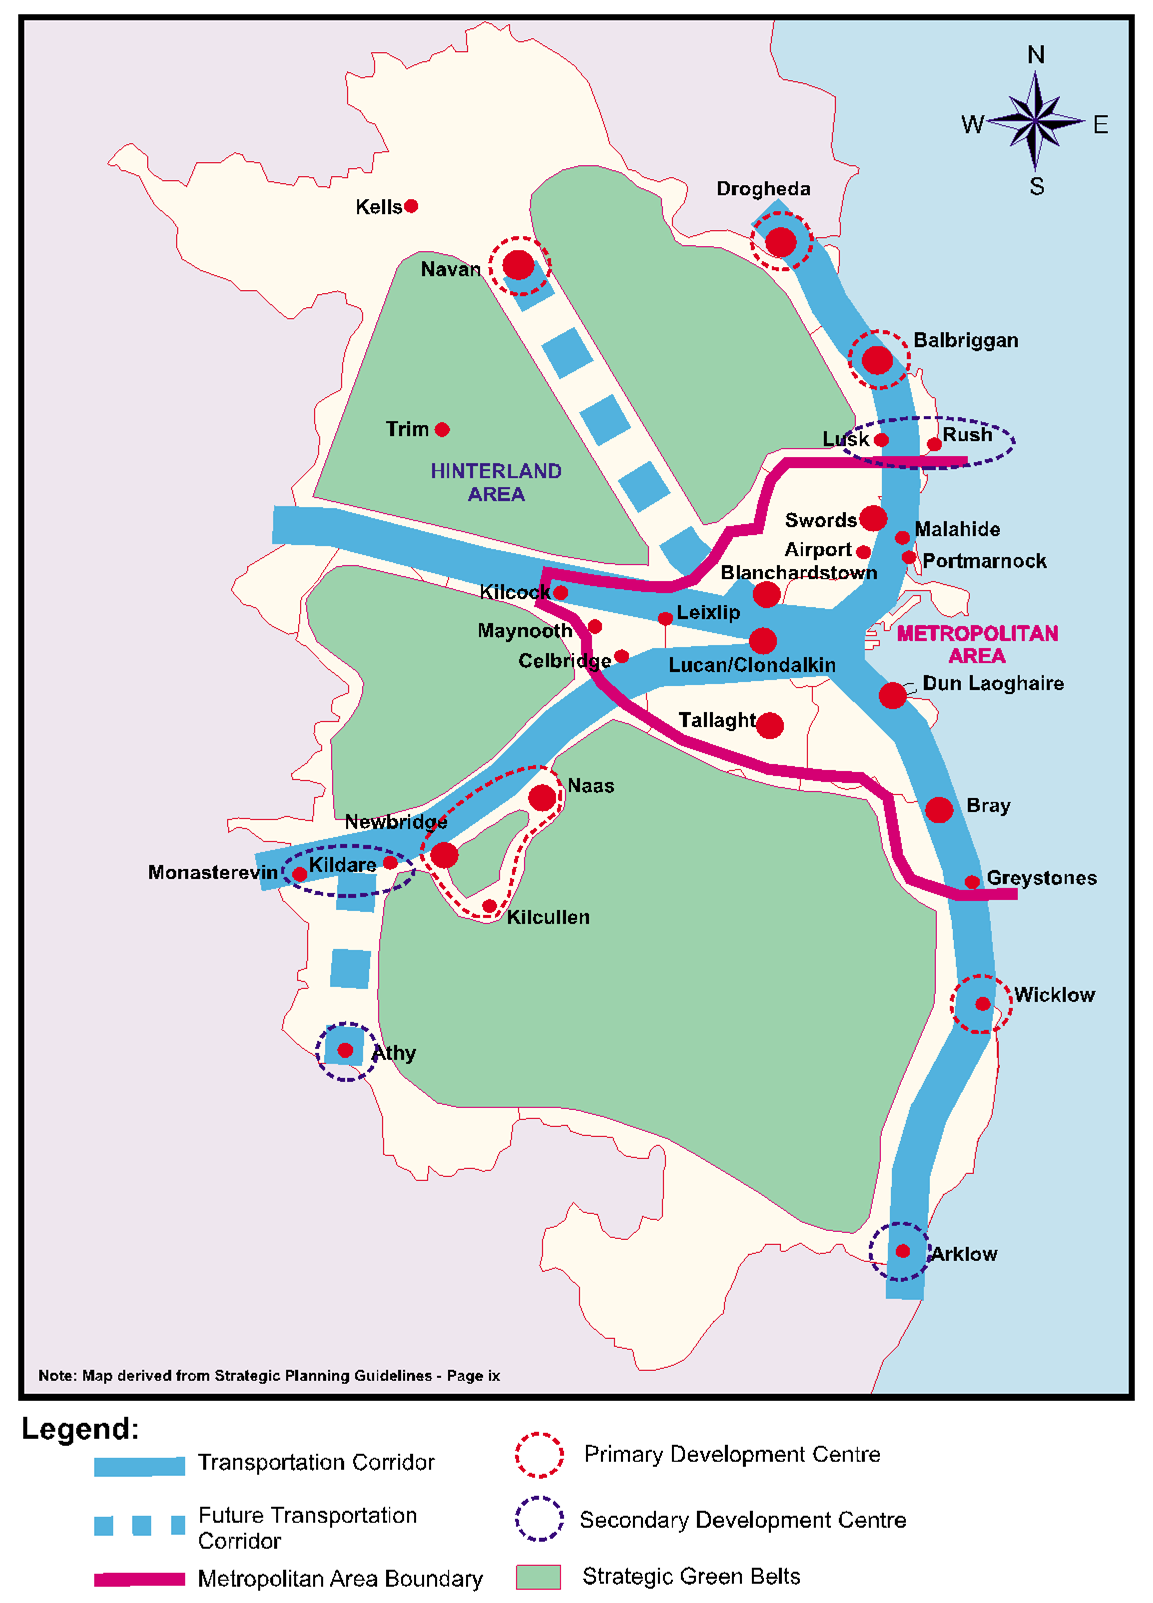
\includegraphics[width=400pt]{intro1}\\
\caption{Map of the Greater Dublin Area \citep{PLA01}} \label{Figure: Map of the Greater Dublin
Area}
\end{figure}
\newpage

\begin{table}[htbp]
\footnotesize{} \setlinespacing{1.0} \vspace{10pt} \begin{longtable} {p{190pt}cccc}
\caption{Demographic Projections of the GDA} \\
\hline

\textbf{Greater Dublin Area}&

\textbf{1991}  & \textbf{1996}& \textbf{1999}& \textbf{2016} \\* \hline \hline {Population
(million) }&

{1.35}  & {1.41}& {1.46}& {1.75} \\* \hline {Households ('000) }&

{402}  & {446}& {521}& {675} \\* \hline {Employment ('000) }&

{452}  & {549}& {681}& {878} \\* \hline {Unemployment rate }&

{16{\%}}  & {12{\%}}& {6{\%}}& {5{\%}} \\* \hline {Car Ownership (per 1000 population)}&

{247}  & {292}& {342}& {480} \\* \hline {{\%} Growth in GDP since 1991}& {- }& {42{\%}}& {79{\%}}&
{260{\%} }\\* \hline

\label{Table: Demographic Projections of the GDA}
\end{longtable}
 \normalsize{} \setlinespacing{1.1}
\end{table}

\newpage

\begin{figure}[htbp]
\center 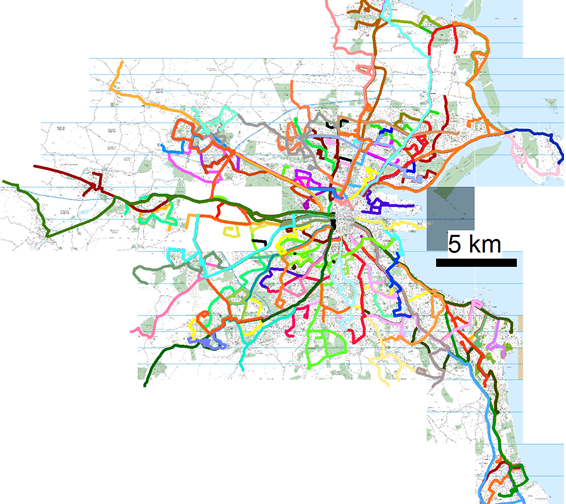
\includegraphics[width=400pt]{intro2}\\
\caption{Map of Bus Routes of Dublin Bus} \label{fig2: Map of bus routes provided by Dublin Bus}
\end{figure}

The figures shown in Table \ref{Table: Demographic Projections of the GDA} are taken from the
website of Dublin Bus \citep{DUB05}. The bus fleet is broken down into depot location and bus
category.

\subsection{Subsection header 2}
fdsdfsdfds
\subsection{Subsection header 3}
fdsdfsdfds
\end{comment}

\section{Justification / Benefits}

\begin{comment}
\subsection{Subsection header 1}
fdsdfsdfds
\subsection{Subsection header 2}
fdsdfsdfds
\subsection{Subsection header 3}
fdsdfsdfds
\end{comment}

When it comes to that time of year where lecturers need to set aside the time to create their examination papers for the modules which they deliver. This is where this project will come into its own with the aim of taking the stress out of the procedure and to provide examiners an easy to use means of examination paper compilation. This usability will come from a combination of a clean and simple user interface along with useful tools to create examination papers.

\section{Feasibility}

\begin{comment}
\subsection{Subsection header 1}

Latex is very good when mathematical formulas need to be displayed:

\begin{equation}\label{taeq2}
    S_{ij}=1-{\frac{|(F_{ij}-F^T_{ij})|}{(F_{ij}+F^T_{ij})}}
\end{equation}


\subsection{Subsection header 2}
\subsection{Subsection header 3}
\end{comment}

Since there are numerous examples of this implementation on the internet. This comes from reading research papers from other students in colleges and technical institutions all around the world. Furthermore the prerequisites obtained from this projects supervisor ensures that the project is technically feasible. However, some research needs to be undertaken regarding the security and encryption aspects. This will be the main technical difficulty and therefore there needs to be a sufficient technical understanding of the technologies involved in order to complete the project.

\section{Proposed Methodologies}

\begin{comment}
\subsection{Subsection header 1}
fdsdfsdfds
\subsection{Subsection header 2}
fdsdfsdfds
\subsection{Subsection header 3}
fdsdfsdfds
\end{comment}

To articulate the methods and techniques used in this plan. Below is the outcome after reviewing various SDLC methodologies with reference to \cite{TP-16}:
\begin{itemize}
	\item Adoption of the Agile Model.
	\item Suits the requirements for this project.
	\item Widely accepted within companies within the IT industry.
	\item Valuable learning curve in gaining experience with this model.
	\item Model has the ability to adapt and tailor itself within each increment as the project moves forward.
	\item Advantageous to the project.
	
\begin{comment}
	\begin{itemize}
		\item A bullet within a bullet!
			\begin{itemize}
				\item Must go deeper...
			\end{itemize}
		\item [Title] Second one too.
	\end{itemize}
	\item Good Things come in threes.
		\item [Title] blah blah blah
		\item [This is a longer title] blah blah blah blah!
			\begin{enumerate}
				\item Some people
				\item Like lists with numbers instead.
			\end{enumerate}
\end{comment}		
\end{itemize}

\begin{comment}
After reviewing the available SDLC methodologies. It has been decided to adopt the Agile Model. Since this best suits the requirements for this project. Adding to this is that it is well recognised as being best practice with companies working within the same field. It would also be a good learning curve in which to gain experience with this model. It can be advantageous to the project as this methodology has the ability to adapt and to tailor itself to each increment of the project as it moves forward.
\end{comment}

\begin{figure}[htbp]
\center 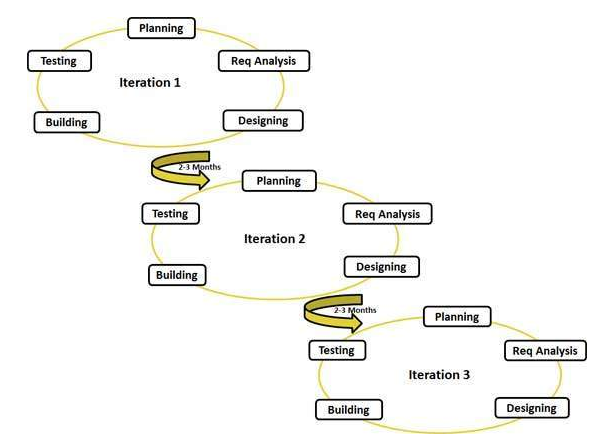
\includegraphics[width=400pt]{Figures/sdlc_agile_model}\\
\caption{Graphical illustration of the Agile Model \citep{TP-16}} \label{Figure: Graphical illustration of the Agile Model}
\end{figure}

\begin{comment}
The diagram shown above \ref{Table: Demographic Projections of the GDA} are taken from the
website of Dublin Bus \citep{TP-16}. The bus fleet is broken down into depot location and bus
category.
\end{comment}

\section{Expected Results}

\begin{comment}
\subsection{Subsection header 1}
fdsdfsdfds
\subsection{Subsection header 2}
fdsdfsdfds
\subsection{Subsection header 3}
fdsdfsdfds
\end{comment}

As noted in the Feasibility section the project should be feasible from a technical standpoint.  It is therefore expected that the project will result in a fully-functioning web site that makes use of the technologies provided.

\section{Conclusion}

\begin{comment}
\subsection{Subsection header 1}
fdsdfsdfds
\subsection{Subsection header 2}
fdsdfsdfds
\subsection{Subsection header 3}
fdsdfsdfds
\end{comment}

This project aims to provide a simple and easy to use service through the use of various Internet technologies combined with automatic generation of question papers and functions. It is hoped that such a service can reduce both the time and difficulties experienced by examiners during an busy time of the year.

\section{Project plan}

\begin{comment}
\subsection{Subsection header 1}
fdsdfsdfds
\subsection{Subsection header 2}
fdsdfsdfds
\subsection{Subsection header 3}
fdsdfsdfds
\end{comment}

Table \ref{table:1} Which shows the Work Breakdown Structure.
 
\begin{table}[h!]
\centering
\begin{tabular}{||c c c c||} 
 \hline
 Task Name & Start & Finish & Duration \\ [0.5ex] 
 \hline\hline
Planning 				& 12/09/16 & 17/10/16 & 42d \\ 
Project Plan 			& 12/09/16 & 26/09/16 & 14d \\
Research Project Ideas	& 12/09/16 & 26/09/16 & 5d \\
Project Proposal 		& 27/09/16 & 12/10/16 & 5d \\
Feasibility Study		& 12/10/16 & 14/10/16 & 13d \\
Research Methodologies 	& 14/09/16 & 16/10/16 & 7d \\
Create Project Proposal   	& 16/10/16 & 26/10/16 & 5d \\
Submit Project Proposal   	& 26/10/16 & 26/10/16 & 0d \\
Literature Review              	& 26/10/16 & 31/10/2016 & 2d \\
Submit Literature Review  & 31/10/2016 & 07/11/2016 & 0d \\
Development                     & 07/11/2016 & 12/12/2016 & 108d \\
Version 1                           	& 12/12/2016 & 12/09/16 & 28d \\
Analysis                            	& 14/09/2016 & 30/09/2016 & 7d \\
User Registration 		& 14/09/2016 & 30/09/2016 & 7d \\
Question Entry 			& 28/10/2016 & 12/09/16 & 7d \\
Create Question Section   & 28/10/2016 & 12/09/16 & 7d \\
Design 				& 28/10/2016 & 31/10/2016 & 7d \\
Use Cases 			& 28/10/2016 & 31/10/2016 & 2d \\
Class Diagrams 		& 31/10/2016 & 07/11/2016 & 2d \\
ERDs 				& 31/10/2016 & 07/11/2016 & 2d \\
Wireframes 			& 31/10/2016 & 07/11/2016 & 1d \\
Implementation 		& 31/10/2016 & 12/09/16 & 14d \\
Database Creation 		& 31/10/2016 & 07/11/2016 & 2d \\
Home Page 			& 31/10/2016 & 07/11/2016 & 3d \\
User Registration 		& 31/10/2016 & 07/11/2016 & 4d \\
Question Entry Page 	& 31/10/2016 & 07/11/2016 & 4d \\
Deliver Version 1 		& 07/11/2016 & 12/12/2016 & 0d \\
Testing 				& 07/11/2016 & 12/12/2016 & 11d \\
Review Version 1 		& 07/11/2016 & 12/12/2016 & 7d \\
Analysis 				& 07/11/2016 & 12/12/2016 & 7d \\
View Listings 			& 07/11/2016 & 12/12/2016 & 7d \\
Show Questions 		& 12/12/2016 & 12/12/2016 & 7d \\
Generate Questions 		& 12/12/2016 & 15/12/2016 & 7d \\
Design 				& 12/12/2016& 15/12/2016 & 7d \\
Use Cases 			& 12/12/2016 & 15/12/2016 & 3d \\
Wireframes 			& 12/12/2016 & 15/12/2016 & 2d \\
ERDs 				& 12/12/2016 & 15/12/2016 & 3d \\
Implementation 		& 09/01/2017 & 15/12/2016 & 14d \\
Database Changes 		& 09/01/2017 & 15/12/2016 & 2d \\
View Questions Page 	& 09/01/2017 & 09/01/2017 & 4d \\
Generate Question Page 	& 09/01/2017 & 09/01/2017 & 4d \\
Testing 				& 09/01/2017 & 09/01/2017 & 12 \\
Deliver Version 2 		& 09/01/2017 & 09/01/2017 & 7d \\
												
 \hline
\end{tabular}
\caption{Table to represent the Work Breakdown Structure}
\label{table:1}
\end{table}

\begin{figure}[htbp]
\center 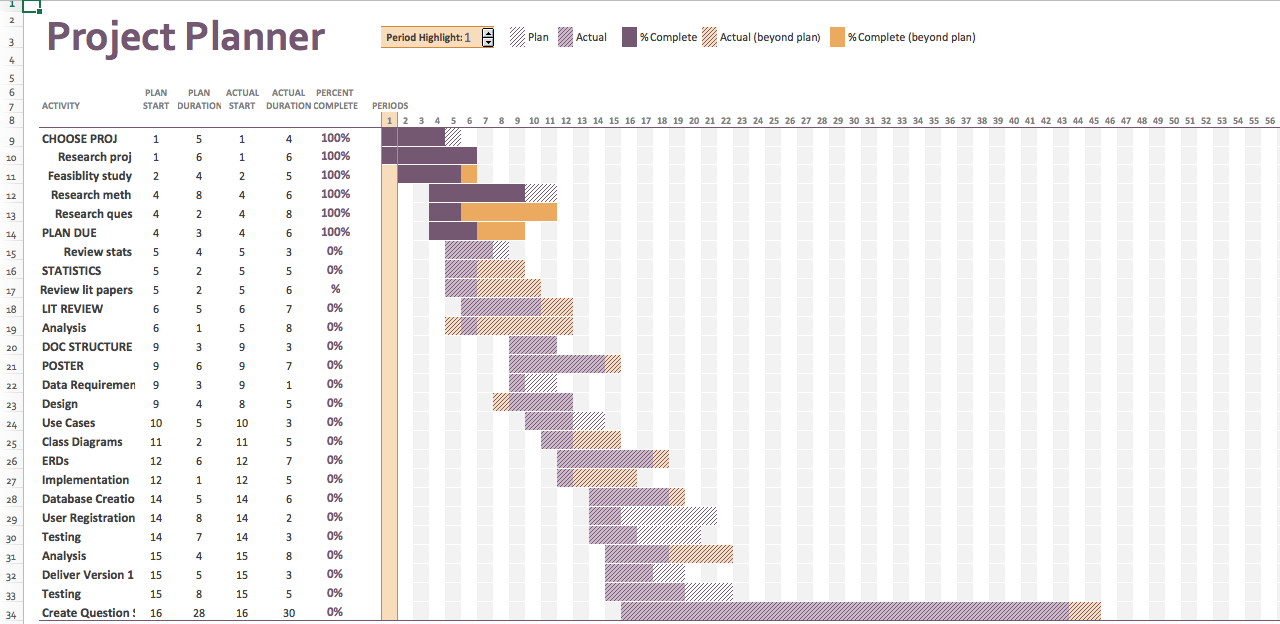
\includegraphics[width=400pt]{Figures/gantt}\\
\caption{Gantt Chart} \label{Figure: Gantt Chart}
\end{figure}

\chapter{Literature Review}


\section{Abstract}

This chapter looks at existing research and development samples undertaken by other students from many countries around the world. These undertakings which have been published were sourced from publishing’s in academic papers, journal articles and books and gathered together from the major works to form part of the research of this narrow topic as they are in the same field of various implementations of random and automatic examination paper generation.


\section{Literature Review}

(Guang Cen, 2010) presented a method to eliminate (Mumbai, 2016) the tradition of the manual composition of examination papers which would usually rely on the writers’ own experience and style of question and knowledge. Although great care would be taken to achieve the best possible outcome of questions with traditional methods there was still the problem of a limited scope of topics and a time consideration. This would bring upon the separation between teaching and creating test papers by means of an automated computer system (Yang Yu, 2008). Comprised of JEE the test system includes modules such as user, subject, question, paper and classification management. Included in this is a question entry and generation module. These modules can be seen in Figure 1 – Schematic diagram of the system function module The question entry and generation makes use of browser and server architecture with a connection to a database of questions. Between this layer is a test server and a WWW server making up the middle layer (Chen, 2008). Figure 2 – Technology road-map of the system shows a flow chart of the system architecture and the use of the MVC pattern with a JSP view, Java Beans, Servlet Controller and a MySQL database (Liu, 2008). The page layout uses divs and CSS technology. In addition to this is support from JavaScript (R. Johnson, 2004). It is the browser which allows the user to choose the subject which they intend on examining. A question type such as student input and a difficulty level. With all these combined parameters, a paper is generated using the generation algorithm (Wang, 2008). This will then be stored in the test database which can be recalled at any stage through system functions for query, or to update the database and for maintenance. It runs in separated modes for user and administrator use. In the end the final document is processed into a Microsoft Word .doc file for distribution in an exam environment. From Figure 3 – Flow chart of the automatic paper generation method it shows how the document is generated.

There are 3 categories which this system falls under. They are, random algorithm based systems, backtracking systems and artificial intelligence and information processing. The first two do not satisfy the specifications (Guiying Deng, 1998). It is the latter which has been improved to avoid the disadvantages of the first and second algorithms. Giving it the ability of searching for questions based on experience and knowledge which guarantees a high standard and quality of examination papers (Hou, 2003). Through using a system with artificial intelligence and information processing the algorithm works quickly and effectively by not selecting a repeated question in a random manner. Questions and answers are separated. It also allowed the user a choice of topics, degree of difficulty, proportion or mark allocation and number of questions per section.

\begin{figure}[htbp]
\center 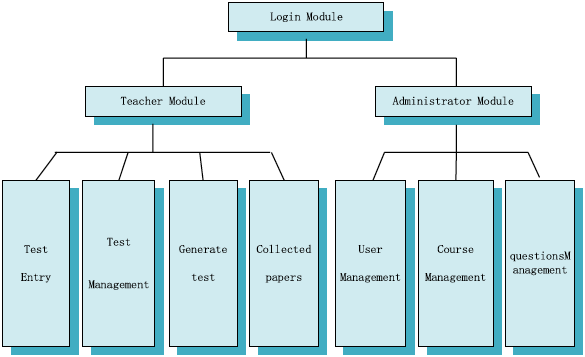
\includegraphics[width=400pt]{Figures/function_module}\\
\caption{Schematic diagram of the system function module \citep{TP-16}} \label{Figure: Schematic diagram of the system function module}
\end{figure}

\begin{figure}[htbp]
\center 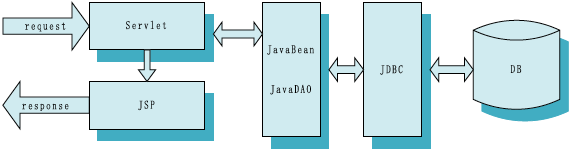
\includegraphics[width=400pt]{Figures/road_map}\\
\caption{Technology road-map of the system \citep{TP-16}} \label{Figure: Technology road-map of the system}
\end{figure}

\begin{figure}[htbp]
\center 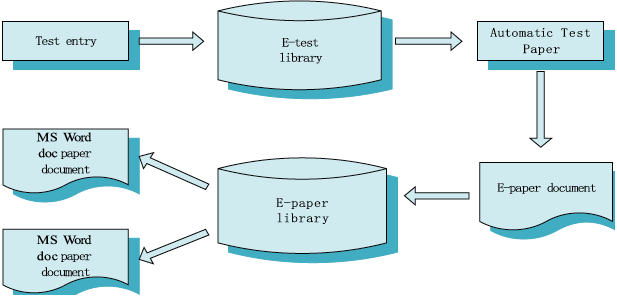
\includegraphics[width=400pt]{Figures/Flow_chart}\\
\caption{Flow chart of the automatic paper generation method \citep{TP-16}} \label{Figure: Flow chart of the automatic paper generation method}
\end{figure}

(Yajuan Zhang, 2011) proposed that although the traditional algorithms in a test paper generation system satisfy the requirements of shuffling the questions. Under certain constraints they do not perform as well as others which have been newly adopted. Here follows a discussion of analysing five intelligent algorithms and how these existing global optimisation algorithms can be integrated into improved shared global optimisation algorithm and dynamic multi branches tree algorithm. These included, improved genetic algorithm, differential evolution algorithm and ant colony optimisation. The particle swarm optimisation algorithm and simulated annealing algorithm. These are divided into two categories which are population evolutionary and others are individual evolutionary and each uses different searching and selection mechanisms. There have been many different studies on trying to improve the algorithms used in terms of speed optimisation however, the improvements were only minor ones. And with the expansion of the system new classifiers need to be constructed for the added samples. The characteristics of the different global optimisation algorithms such as the improved genetic algorithm. Based on the genetic algorithm with modifications such as improvements to integer coding which displays higher search speeds performing well and is very practical. It also avoids prematurity which occurs in the genetic algorithm. The genetic algorithm performs a randomised search simulating natural selection and genetic variation to problem solve. With the disadvantage of having a low search efficiency with premature convergence. The differential evolution algorithm is simple and effective in that the population size remains unchanged throughout the operation process. These operations include variation, crossover and selection with advances such as simple principle, control parameters, robustness a high convergence rate and straightforward realisation. The ant colony algorithm simulates an ant colony and their routing behaviours in nature. Finding a solution through information exchange and cooperation among the ant colony. However, the mechanism for feedback has a slow convergence speed. The particle swarm optimisation algorithm has good performance however, needs to be used indirectly in getting the optimal solution of multiple object optimisation problems. As during a search its own position needs to be updated through a follow up of individual extreme value and global extreme value. Simulated annealing algorithm finds the probability sense using a random search. Which is a global optimisation method.
(Dan Liu, 2013) derived a method for test paper generation through using the ant colony algorithm. A comparison is also made between using other algorithms such as a random variable algorithm a backtracking algorithm and an artificial intelligence algorithm. Describing the random variable algorithm is that is extracts questions and if they meet certain conditions it then forms a test paper based on these conditions. However, it can fail to meet these requirements. Which in turn offers a poor success rate. The backtracking algorithm works well on small scale generation. Once the scale is largely increased so the time taken to process the generation increases. A new approach would be to compose test papers using the ant colony algorithm as it can search at a far greater speed with and intelligent search.

\chapter{Methodology Chapter}


\section{Introduction}

Agile is not a methodology but more of an alternative to the existing SDLC Models. To articulate the methods and techniques used in this plan. In figure \ref{fig:agile} is the outcome after reviewing various SDLC methodologies with reference to \cite{TP-16}:
\begin{itemize}
	\item Adoption of the Agile Model.
	\item Suits the requirements for this project.
	\item Widely accepted within companies within the IT industry.
	\item Valuable learning curve in gaining experience with this model.
	\item Model has the ability to adapt and tailor itself within each increment as the project moves forward.
	\item Advantageous to the project.
\end{itemize}

\begin{figure}[Htbp]
\center 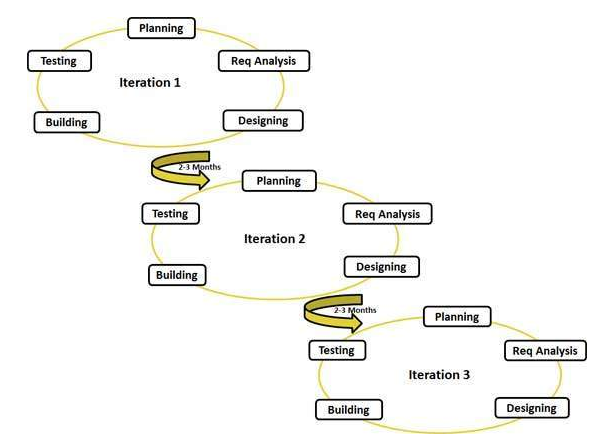
\includegraphics[width=400pt]{Figures/sdlc_agile_model}\\
\caption{Graphical illustration of the Agile Model \citep{TP-16}} \label{Figure: Graphical illustration of the Agile Model}
\label{fig:agile}
\end{figure}	

\subsection{What is Agile?}
Agile is an iterative approach to software delivery that builds software incrementally from the start of the project, instead of trying to deliver it all at once near the end. It works by breaking projects down into little bits of user functionality called user stories, prioritizing them, and then continuously delivering them in short two week cycles called iterations.

\begin{figure}[htbp]
\center 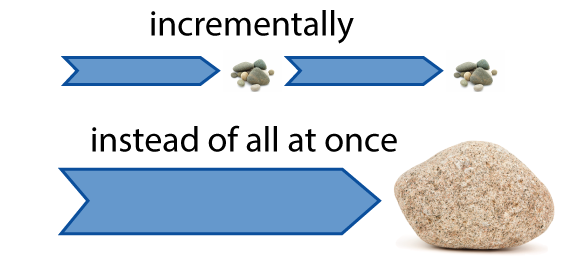
\includegraphics[width=400pt]{figures/incrementally-over-all-at-once}\\
\caption{Increments of the Agile Model \citep{AIAN-16}} \label{Figure: Increments of the Agile Model}
\label{fig:agile}
\end{figure}

\begin{figure}[htbp]
\center 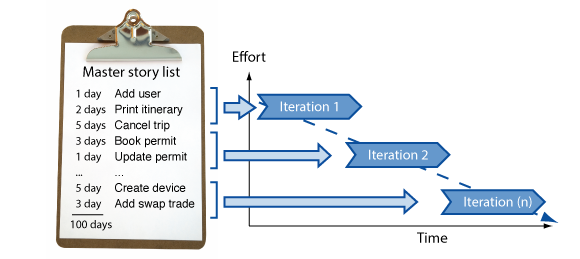
\includegraphics[width=400pt]{figures/burn-down-simple}\\
\caption{Iterations of the Agile Model \citep{AIAN-16}} \label{Figure: Iterations of the Agile Model}
\label{fig:agile}
\end{figure}

\subsection{How does it work?}
At its core, Agile does the same thing you and I do when faced with too much to do and not enough time. Then, using Agile estimation techniques, you size your stories relatively to each other, coming up with a guess as to how long you think each user story will take. Like most lists, there always seems to be more to do than time allows. So you ask your customer to prioritize their list so you get the most important stuff done first, and save the least important for last. Then you start delivering some value. You start at the top. Work your way to the bottom. Building, iterating, and getting feedback from your customer as you go. Then, as you and your customer starting delivering, one of two things is going to happen. You'll discover:

    You're going fast enough. All is good. Or,
    You have too much to do and not enough time.

At this point you have two choices. You can either a) do less and cut scope (recommended). Or you can b) push out the date and ask for more money.

\begin{figure}[htbp]
\center 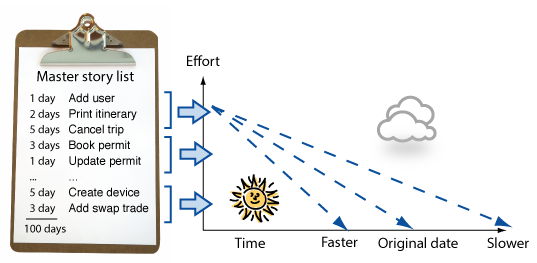
\includegraphics[width=400pt]{figures/update-the-plan}\\
\caption{Making a list \citep{AIAN-16}} \label{Figure: Making a list}
\label{fig:agile}
\end{figure}

\subsection{How is it different?}
Analysis, design, coding, and testing are continuous activities

You are never done analysis, design, coding and testing on an Agile project. So long as there are features to build, and the means to deliver them, these activities continue for the duration of the project.

\subsection{Agile vs Waterfall}
Traditional Waterfall treats analysis, design, coding, and testing as discrete phases in a software project. This worked OK when the cost of change was high. But now that it's low it hurts us in a couple of ways. First off, when the project starts to run out of time and money, testing is the only phase left. This means good projects are forced to cut testing short and quality suffers. Secondly, because working software isn't produced until the end of the project, you never really know where you are on a Waterfall project. That last 20\% of the project always seems to take 80\% of the time.

\section{Data Collection Methods}

\subsection{Internet Search}
Discusses where I obtained my information
\subsection{Supervisor Input}
Discussion on how to store the encrypted data in tables 
\subsection{Journals in Library}
Journals which were read and relevant to this project


\section{Method of Analysis}

\subsection{Formulation of Where to Start}
Researching the title of the project
\subsection{Early System Implementation}
This project was linked to an assignment which helped in my progression
\subsection{Review of Literature}
Undertaking a literature review aided with making comparisons of other systems produced


\section{Summary}

Summary with all terms discussed within the chapter
\begin{comment}
\subsection{Subsection header 1}
fdsdfsdfds
\subsection{Subsection header 2}
fdsdfsdfds
\subsection{Subsection header 3}
fdsdfsdfds
\end{comment}

\chapter{Implementation - "Building the solution"}


\section{Introduction}

This chapter is a walkthrough of the steps which describe the construction of the application.

\section{Terminal}

\subsection{Command Line Instructions}

As this application was centred towards security and being secure as the data it would hold would need to be kept safe. Therefore it made sense to focus on a good login with authentication and authorisation. To start working with Symfony, one needs to setup the Symfony enviroment through an installation process before Symfony applications can be created. Instructions for this can be found on the SensioLabs Symfony website. Navigating to the Documentation page. In there can be found Chapter 1 which has the Setup instructions under the Get Started dropdown menu. They explain the different ways for installing and setting up the Symfony framework for both Mac OS and Windows. Along with some\newline troubleshooting ideas if there are any problems with the installation. This application was built on a Mac OS so the instructions would vary slightly due to the command line instructions used. Using the installer made it easy to create this application with Symfony and only needed to be done once as it was installed globally on the machine.

\begin{figure}[htbp]
   \centering
   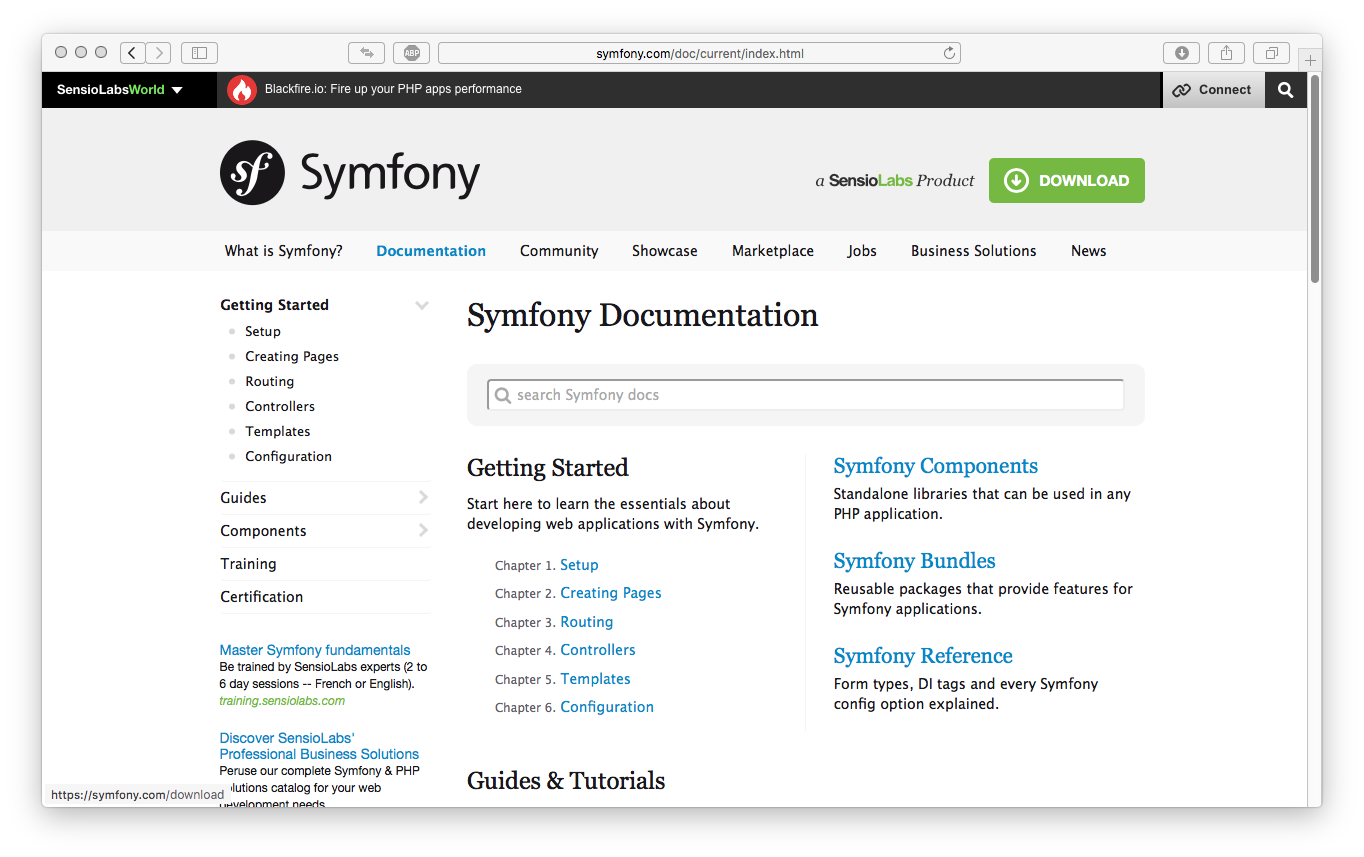
\includegraphics[width=400pt]{figures/symfony_documentation.png} % requires the graphicx package
   \caption{Symfony Documentation}
   \label{fig:Symfony Documentation}
\end{figure}

\begin{figure}[htbp]
   \centering
   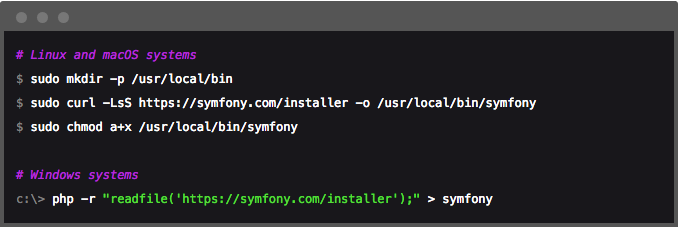
\includegraphics[width=400pt]{figures/symfony_installation.png} % requires the graphicx package
   \caption{Symfony Installation Setup}
   \label{fig:Symfony Installation Setup}
\end{figure}

With this completed moving into the directory or environment that the application will live which was the desktop. A final command in the terminal window was issued. This time starting with symfony new and by giving a project a name of choice thereafter. In this case the name COMPH4021-Project was used. The project was based on the current version of Symfony which is version 3.2.8. However, other versions can be specified after the project name in the terminal window. Once this part was completed. All required components were downloaded into a project folder with the name of which was given. The components are a set of files and directories which form the web application which use the Symfony libraries. The installer also carries out a check to make sure all requirements are met. If requirements are not all met a list is generated which provides the changes that are needed. In this case no changes needed to be made.

\begin{figure}[htbp]
   \centering
   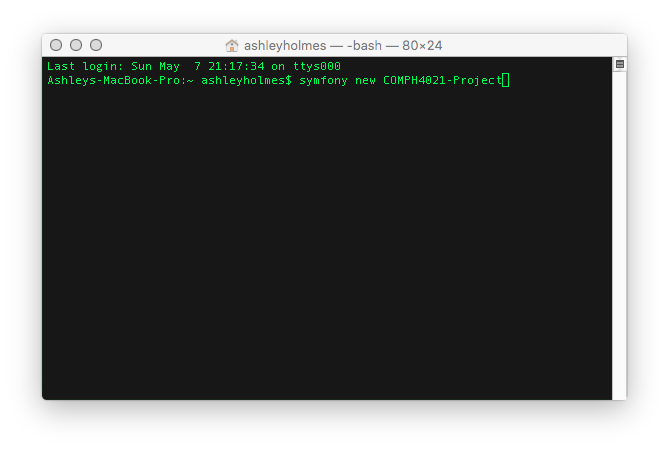
\includegraphics[width=400pt]{figures/new_application.png} % requires the graphicx package
   \caption{Symfony Application Setup}
   \label{fig:Symfony Application Setup}
\end{figure}

The below figure \ref{fig:Terminal Window Top} displays the command issued to download the project folder and following that in figure \ref{fig:Terminal Window Bottom} one can see that the project is being prepared and where it will be stored. In this case it was stored in /Users/ashleyholmes/Desktop/COMPH4021-Project.

\begin{figure}[htbp]
   \centering
   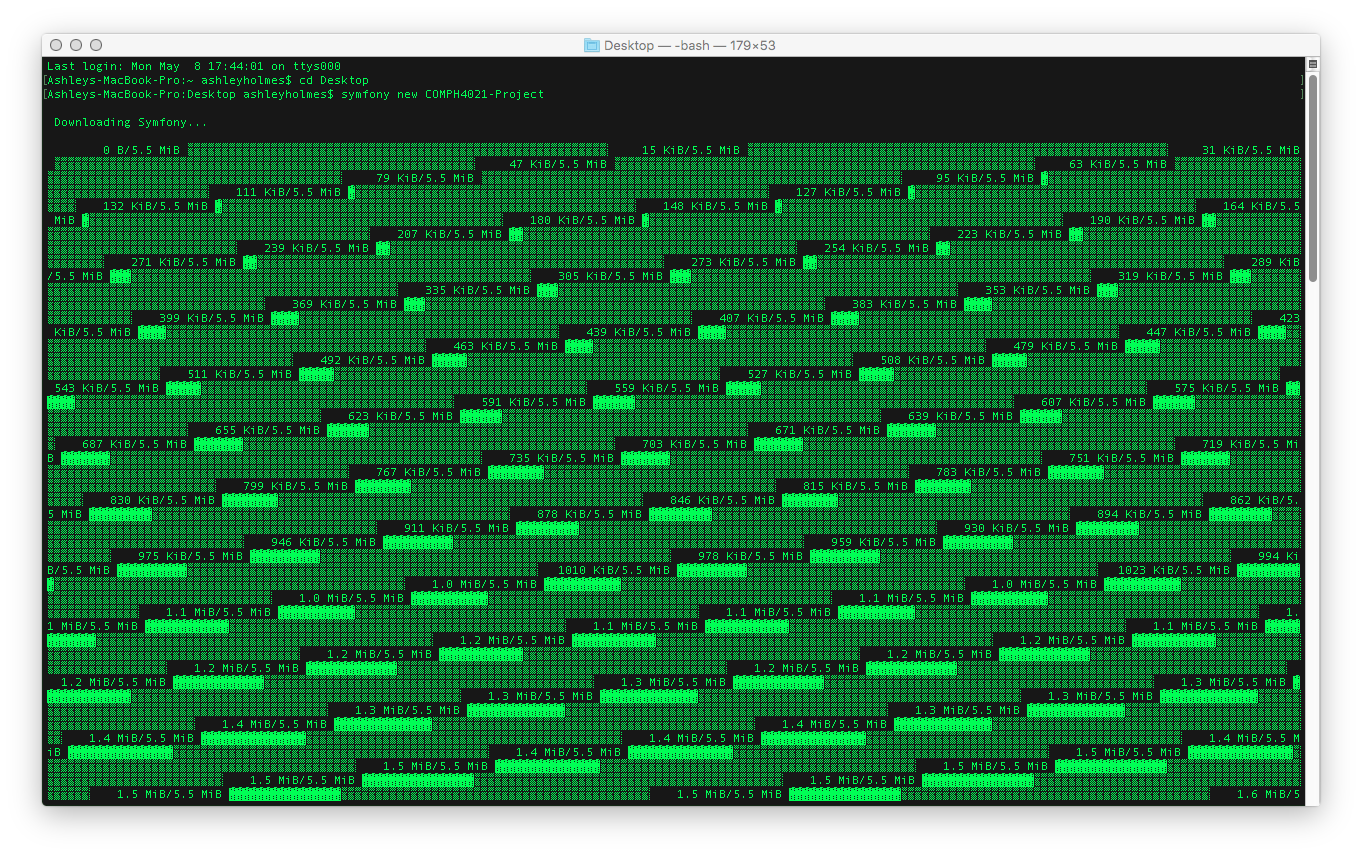
\includegraphics[width=400pt]{figures/terminal_window_top.png} % requires the graphicx package
   \caption{Terminal Window Top}
   \label{fig:Terminal Window Top}
\end{figure}

\begin{figure}[htbp]
   \centering
   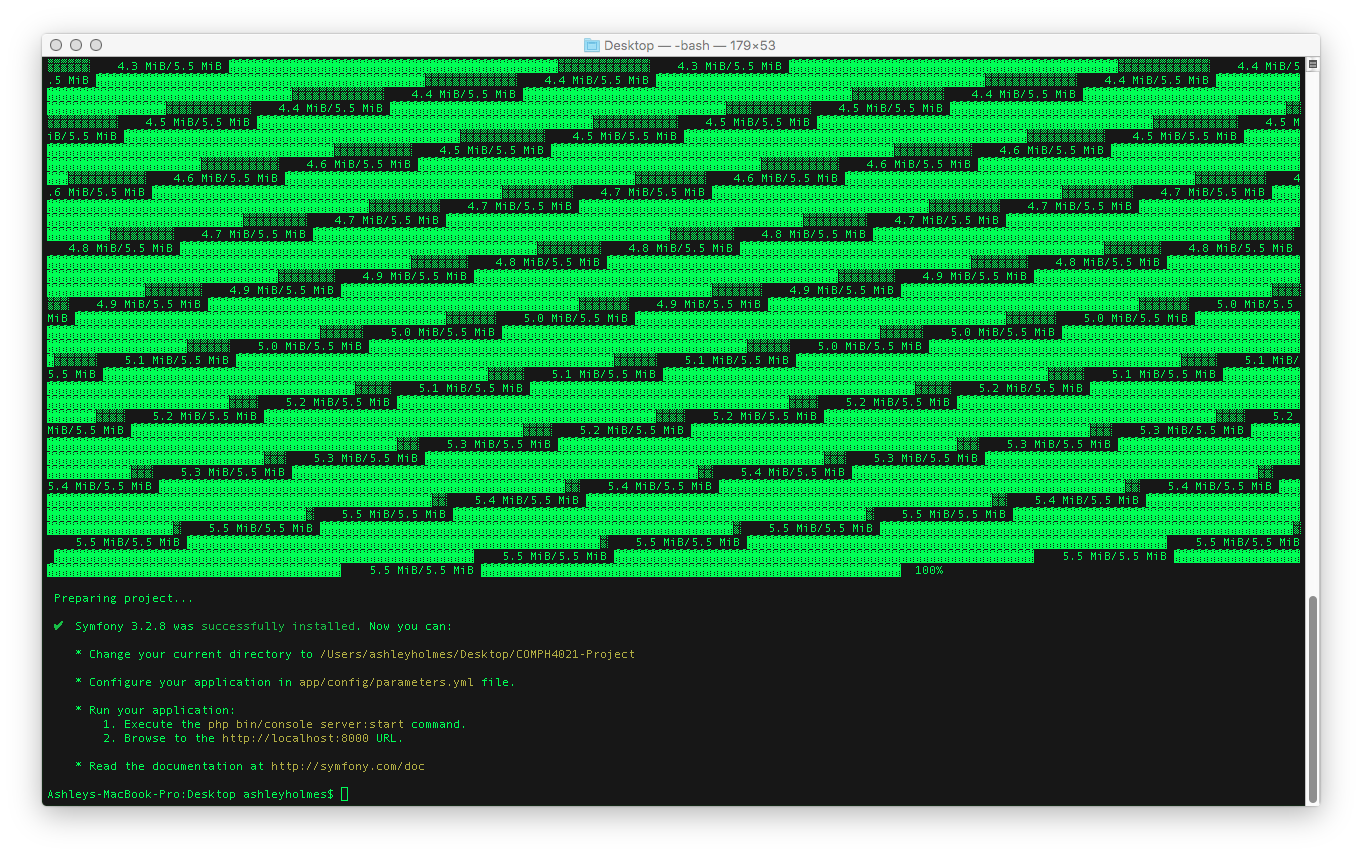
\includegraphics[width=400pt]{figures/terminal_window_bottom.png} % requires the graphicx package
   \caption{Terminal Window Bottom}
   \label{fig:Terminal Window Bottom}
\end{figure}

\begin{figure}[htbp]
   \centering
   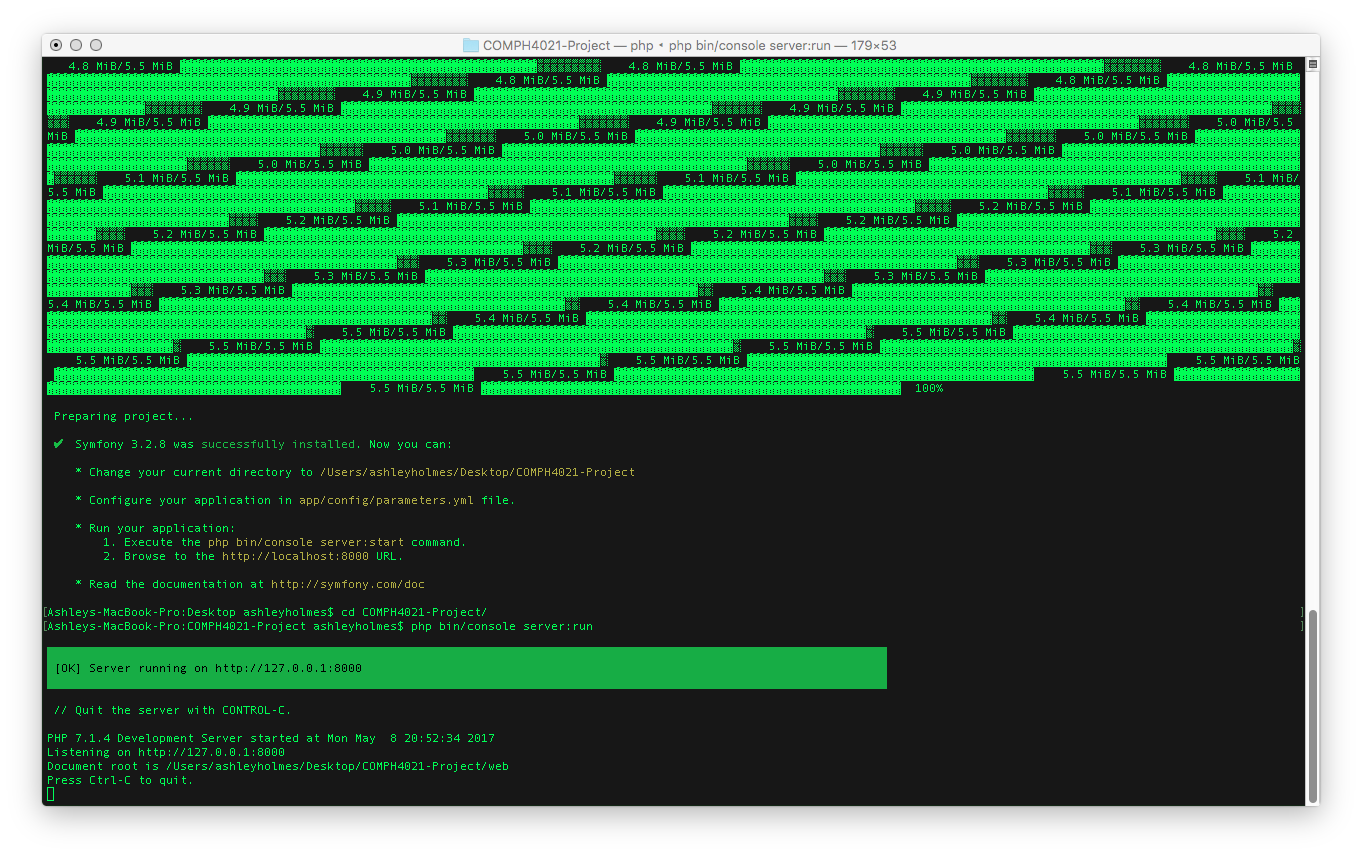
\includegraphics[width=400pt]{figures/php_server_run.png} % requires the graphicx package
   \caption{Php Server Run}
   \label{fig:Php Server Run}
\end{figure}

\begin{figure}[htbp]
   \centering
   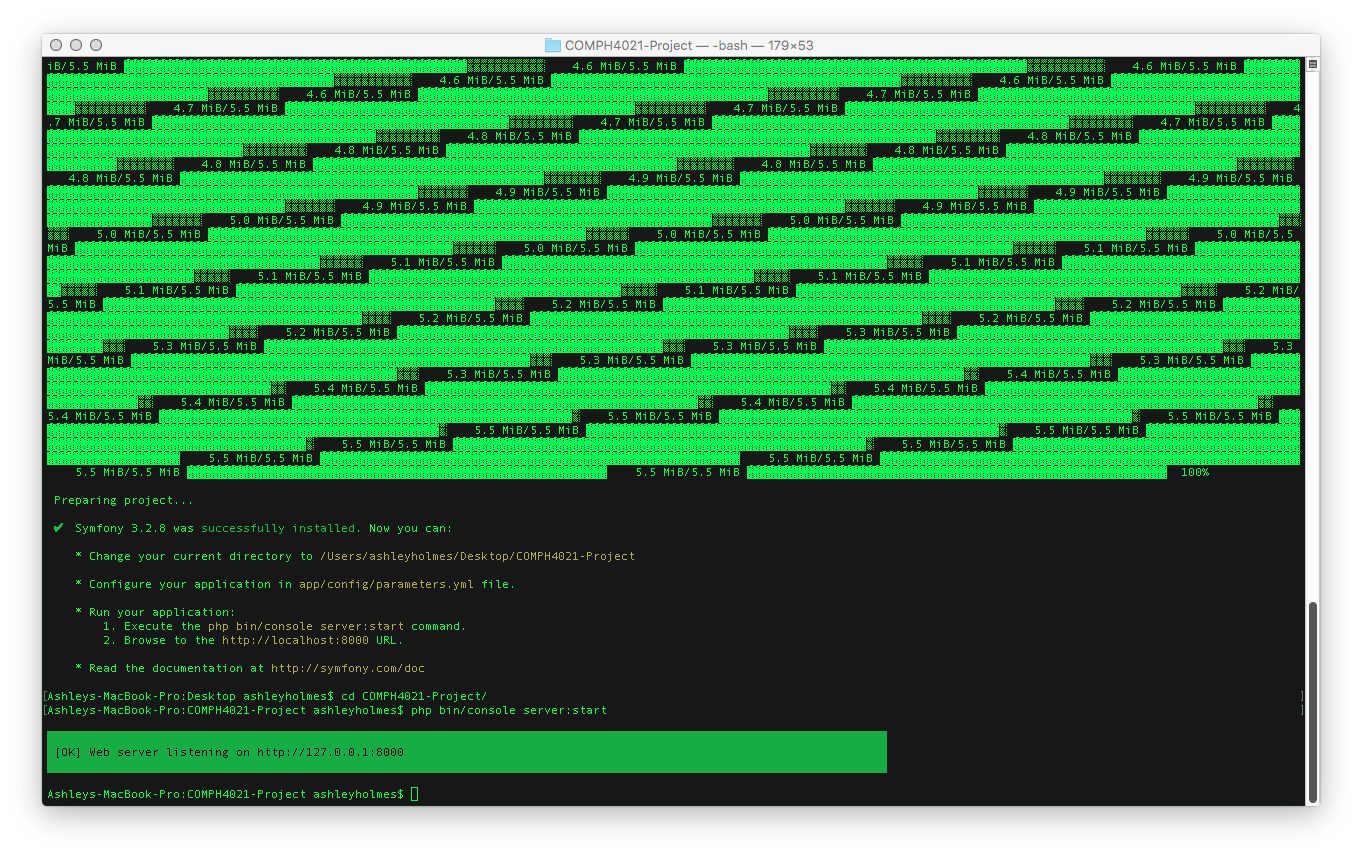
\includegraphics[width=400pt]{figures/php_server_start.png} % requires the graphicx package
   \caption{Php Server Start}
   \label{fig:Php Server Start}
\end{figure}

The next step would be to change directory into the COMPH4021-Project directory as this is where the built in Php server needs to be run from. NGINX and Apache may be used as alternatives however, since the Php server is built in. It makes development much easier. Executing the following command php bin/console server:run starts the server. However, once issuing this command the open terminal window would now need to remain out of use while the server is running. One can use a separate terminal window or open a new tab to issue any addition commands which are needed or make use of the PhpStorm terminal window. To run other processes in the background, issuing a php bin/console server:start will make it possible to execute commands in the same window which was done here. The difference can be seen in figure \ref{fig:Php Server Run} and figure \ref{fig:Php Server Start}.

\section{Browser}

\subsection{Deploying the Application}

\begin{figure}[htbp]
   \centering
   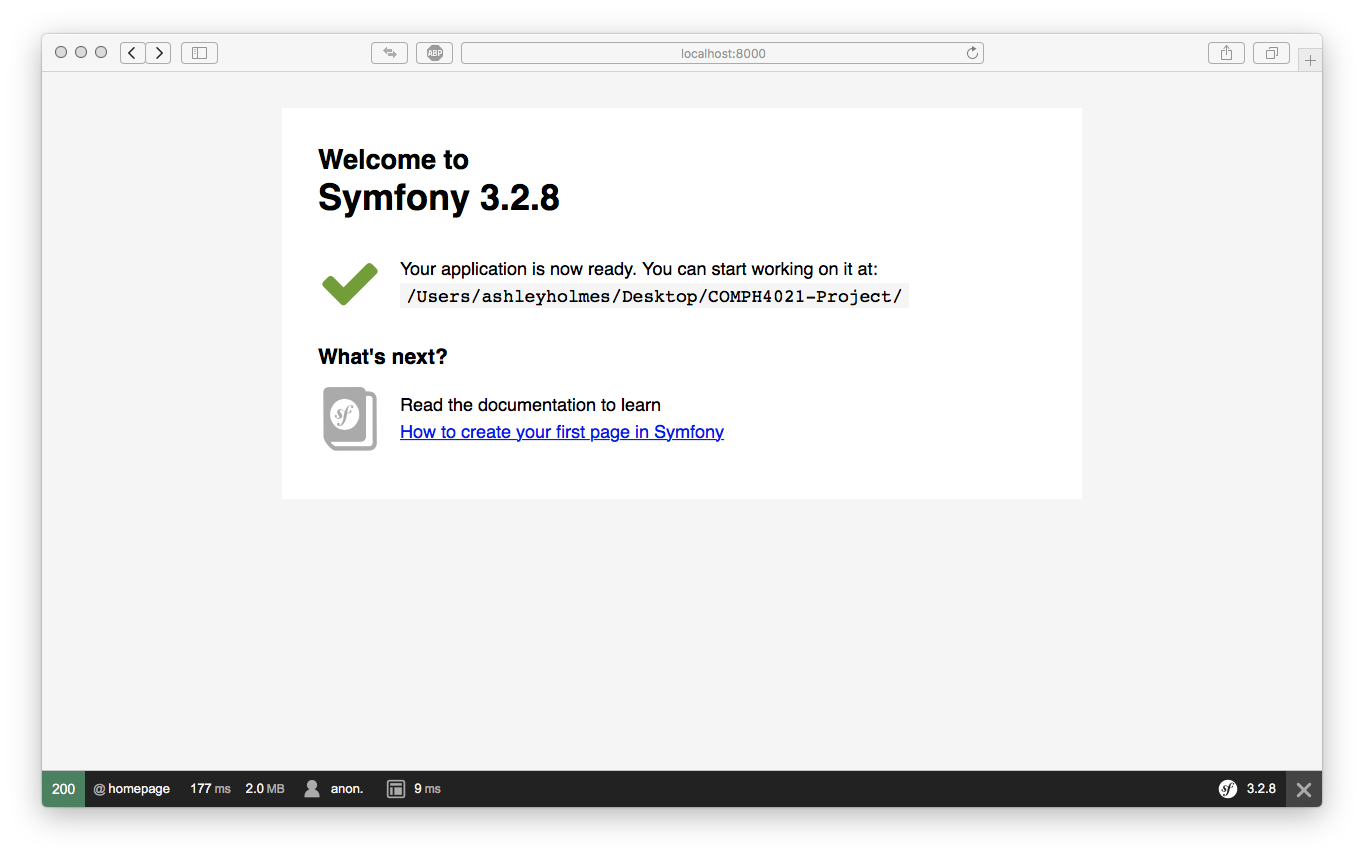
\includegraphics[width=400pt]{figures/symfony_browser.png} % requires the graphicx package
   \caption{Symfony Browser}
   \label{fig:Symfony Browser}
\end{figure}

\begin{figure}[htbp]
   \centering
   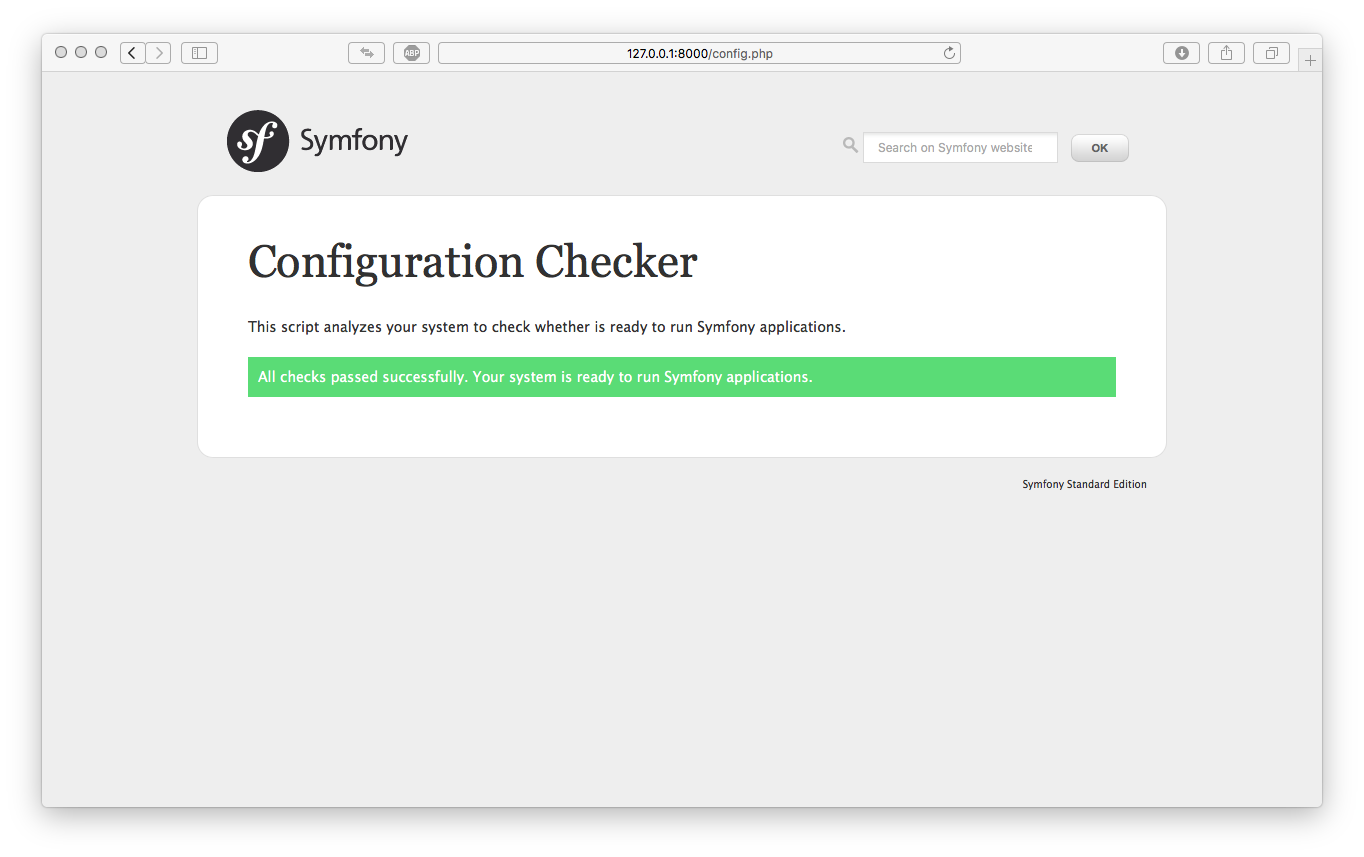
\includegraphics[width=400pt]{figures/configuration_checker.png} % requires the graphicx package
   \caption{Configuration Checker}
   \label{fig:Configuration Checker}
\end{figure}

\begin{figure}[htbp]
   \centering
   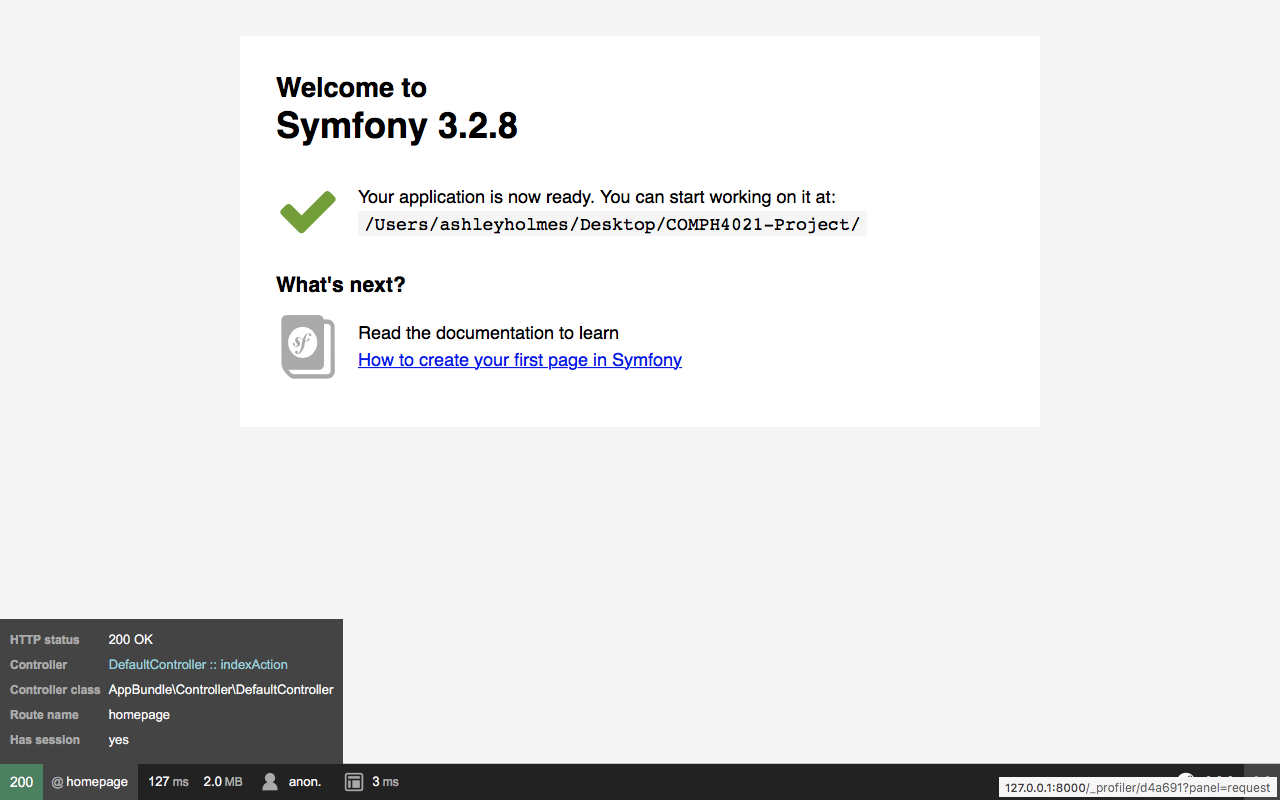
\includegraphics[width=400pt]{figures/webdebug_1.png}
   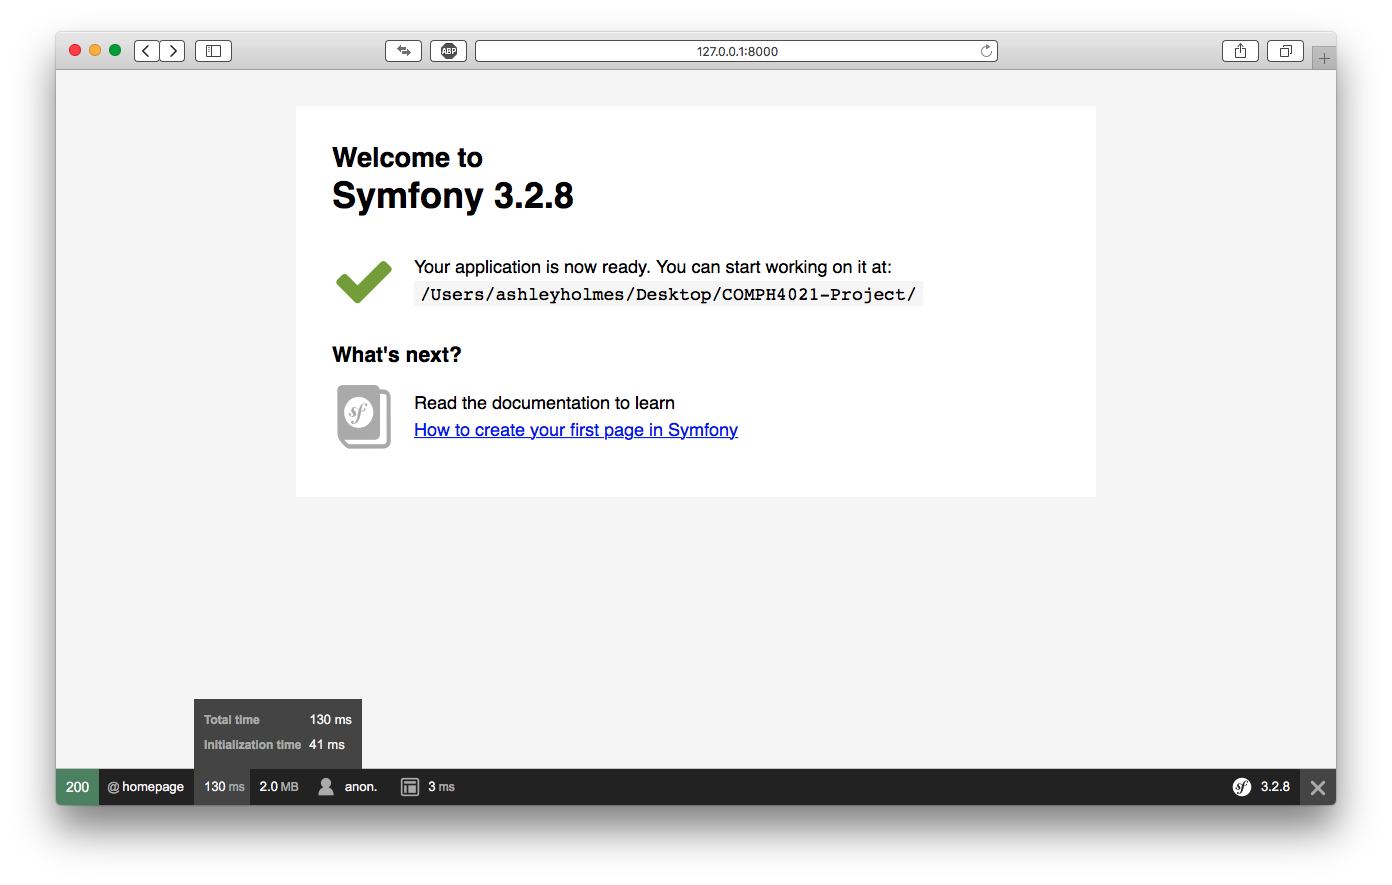
\includegraphics[width=400pt]{figures/webdebug_2.png} % requires the graphicx package
   \caption{Web Debug Toolbar and Profiler Extended}
   \label{fig:Web Debug Toolbar and Profiler Extended}
\end{figure}

\begin{figure}[htbp]
   \centering
   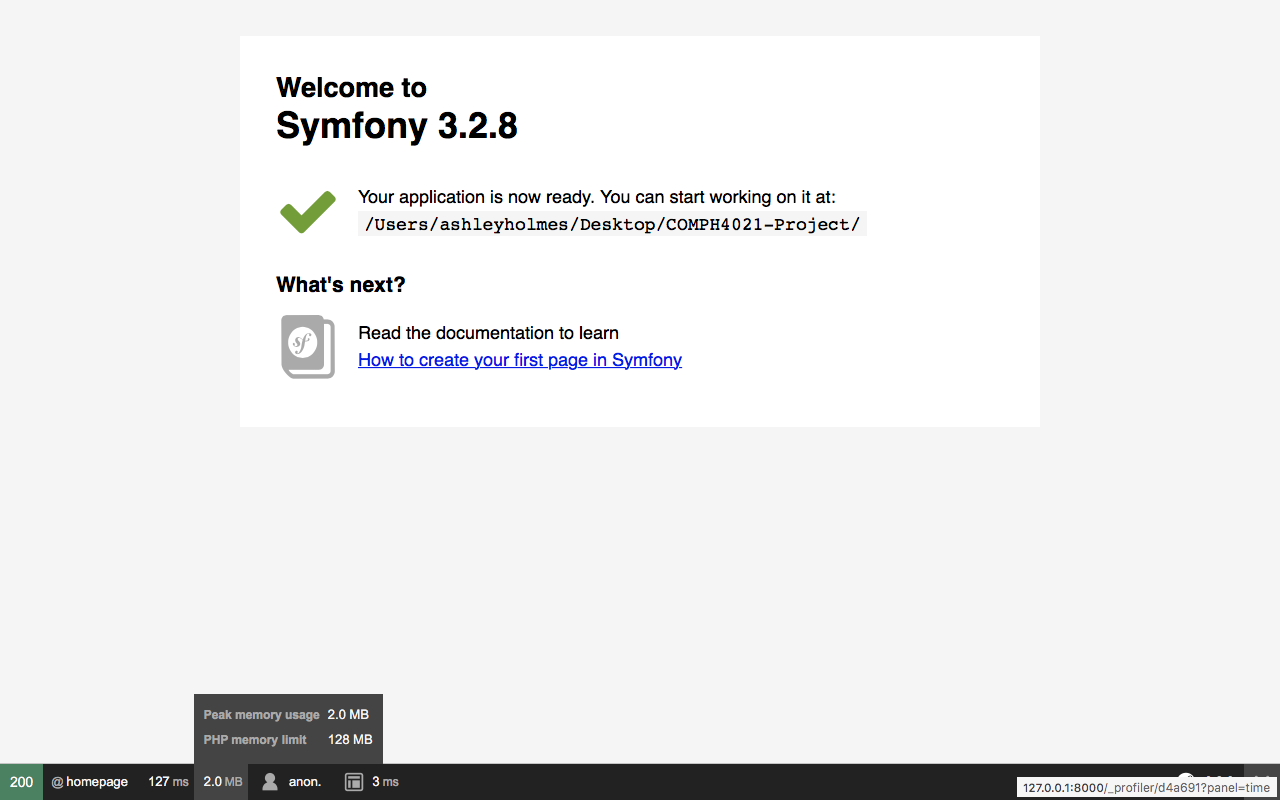
\includegraphics[width=400pt]{figures/webdebug_3.png} % requires the graphicx package
   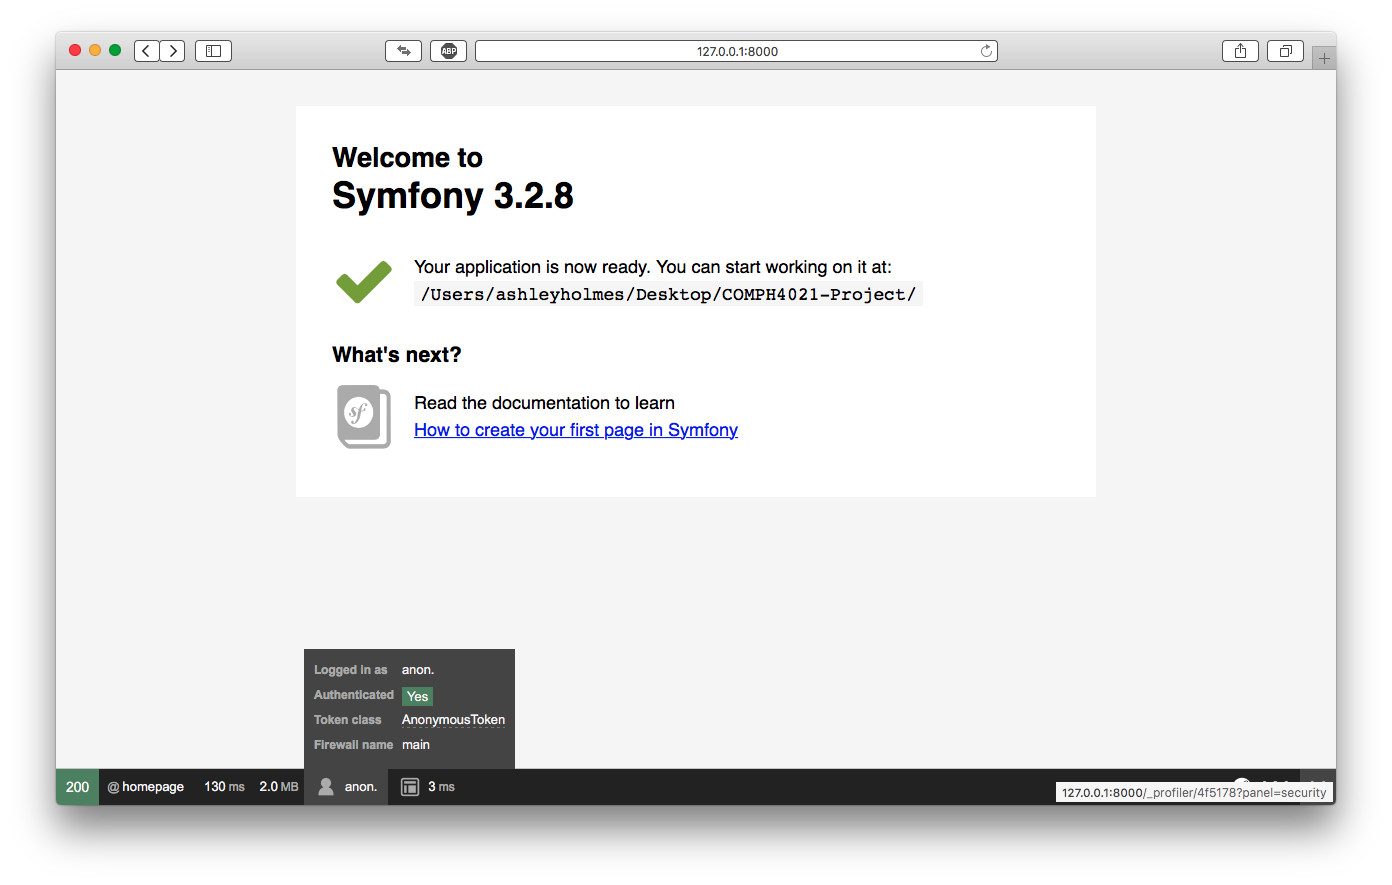
\includegraphics[width=400pt]{figures/webdebug_4.png}
   \caption{Web Debug Toolbar and Profiler Extended}
   \label{fig:Web Debug Toolbar and Profiler Extended}
\end{figure}

\begin{figure}[htbp]
   \centering
   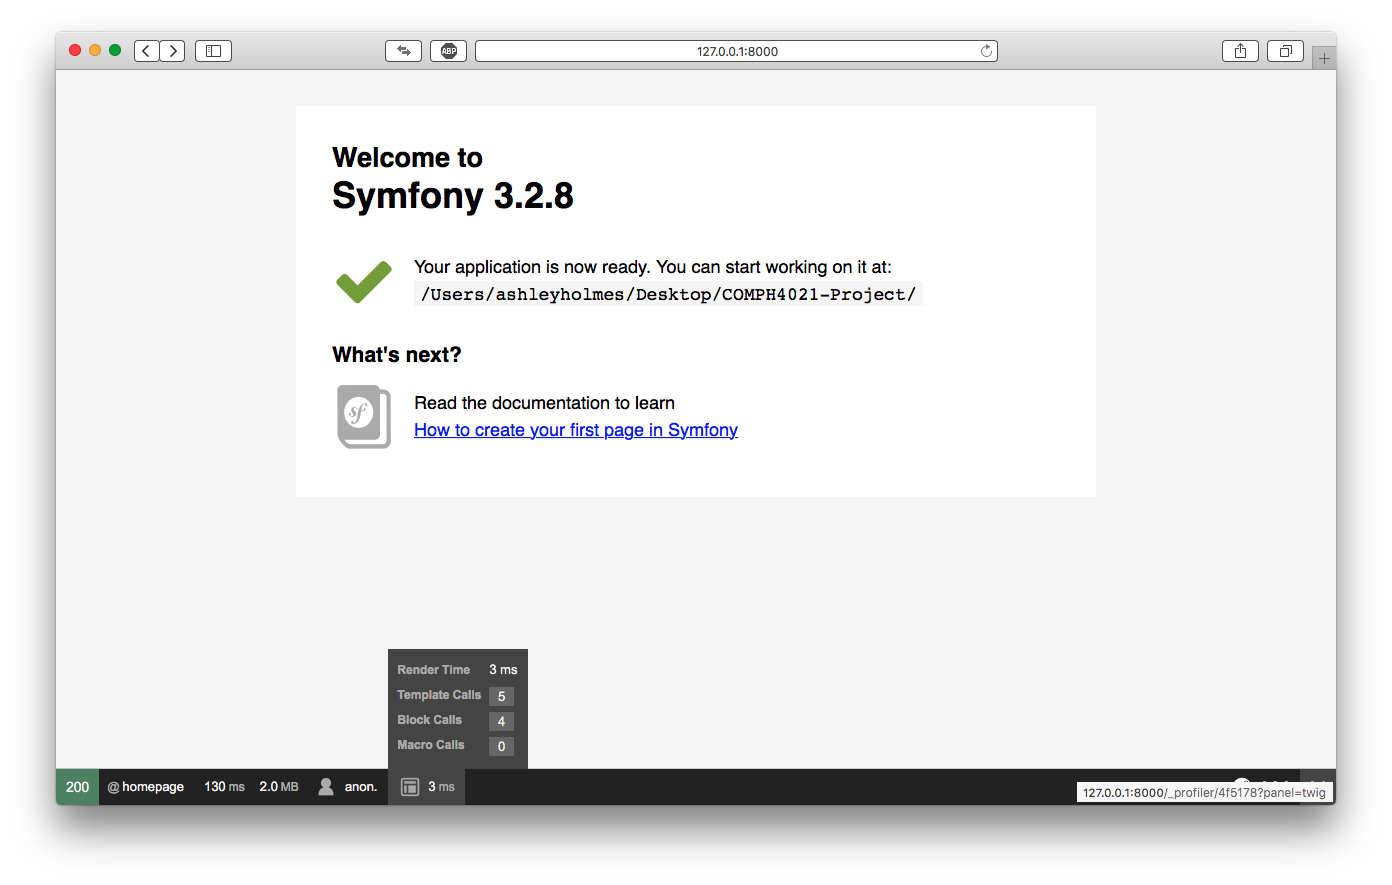
\includegraphics[width=400pt]{figures/webdebug_5.png}
   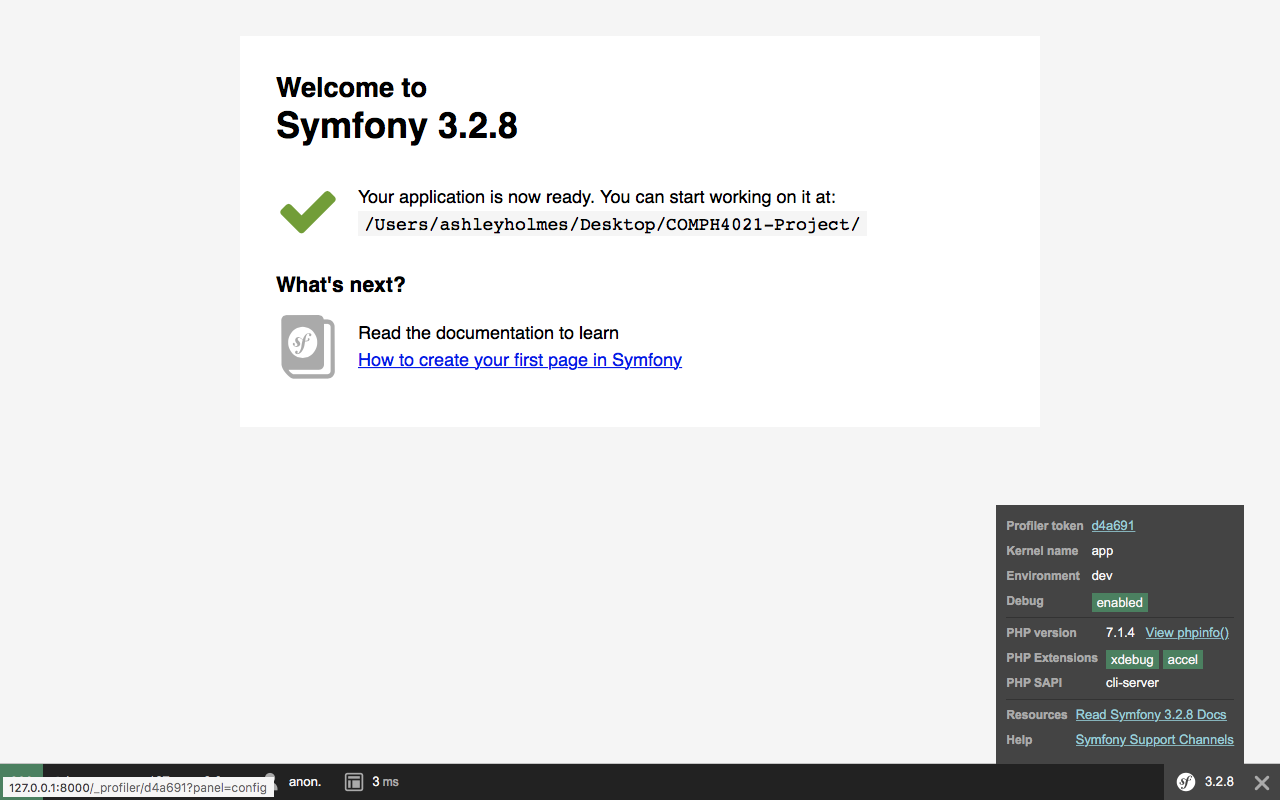
\includegraphics[width=400pt]{figures/webdebug_6.png} % requires the graphicx package
   \caption{Web Debug Toolbar and Profiler Extended}
   \label{fig:Web Debug Toolbar and Profiler Extended}
\end{figure}

Now that the configuration phase has been completed one now navigates to the browser and using the URL http://localhost:8000 as shown in the terminal window in figure \ref{fig:Terminal Window Bottom} under the Run your application heading. This brings up the following page in figure \ref{fig:Symfony Browser}. It is being executed by the Symfony framework from the files inside the project folder. The code is depicted in figure \ref{fig:Web Debug Toolbar and Profiler}. In the bottom of the window is the web debug toolbar which is in a maximised position and can be minimised by clicking on the X in the right hand corner. This often offers better visibility when developing. If the mouse is used to hover over the toolbar it will display information such as routing, controllers which were executed, time it took to load the page, which way the user is authenticated on the page and more debugging information and a link to the resources and documentation as shown in figure \ref{fig:Web Debug Toolbar and Profiler Extended}. Clicking on the icons will give much more information. The URL http://127.0.0.1:8000/config.php would show the user the instructions needed for further configuration. This is reference to figure \ref{fig:Configuration Checker}.


\begin{figure}[htbp]
   \centering
   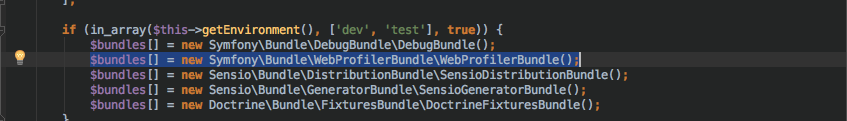
\includegraphics[width=400pt]{figures/AppKernel.png}
   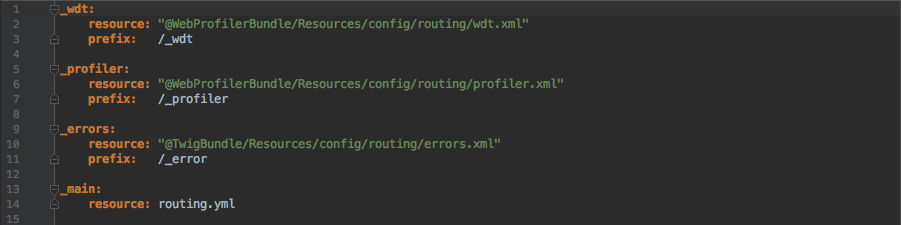
\includegraphics[width=400pt]{figures/routing_dev.png}
   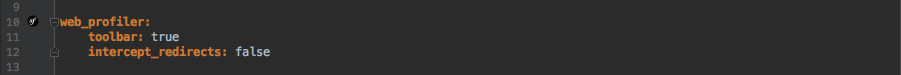
\includegraphics[width=400pt]{figures/config_dev.png} % requires the graphicx package
   \caption{Web Debug Toolbar and Profiler}
   \label{fig:Web Debug Toolbar and Profiler}
\end{figure}

\section{IDE}

\subsection{PhpStorm IDE for PHP}

\begin{figure}[htbp]
   \centering
   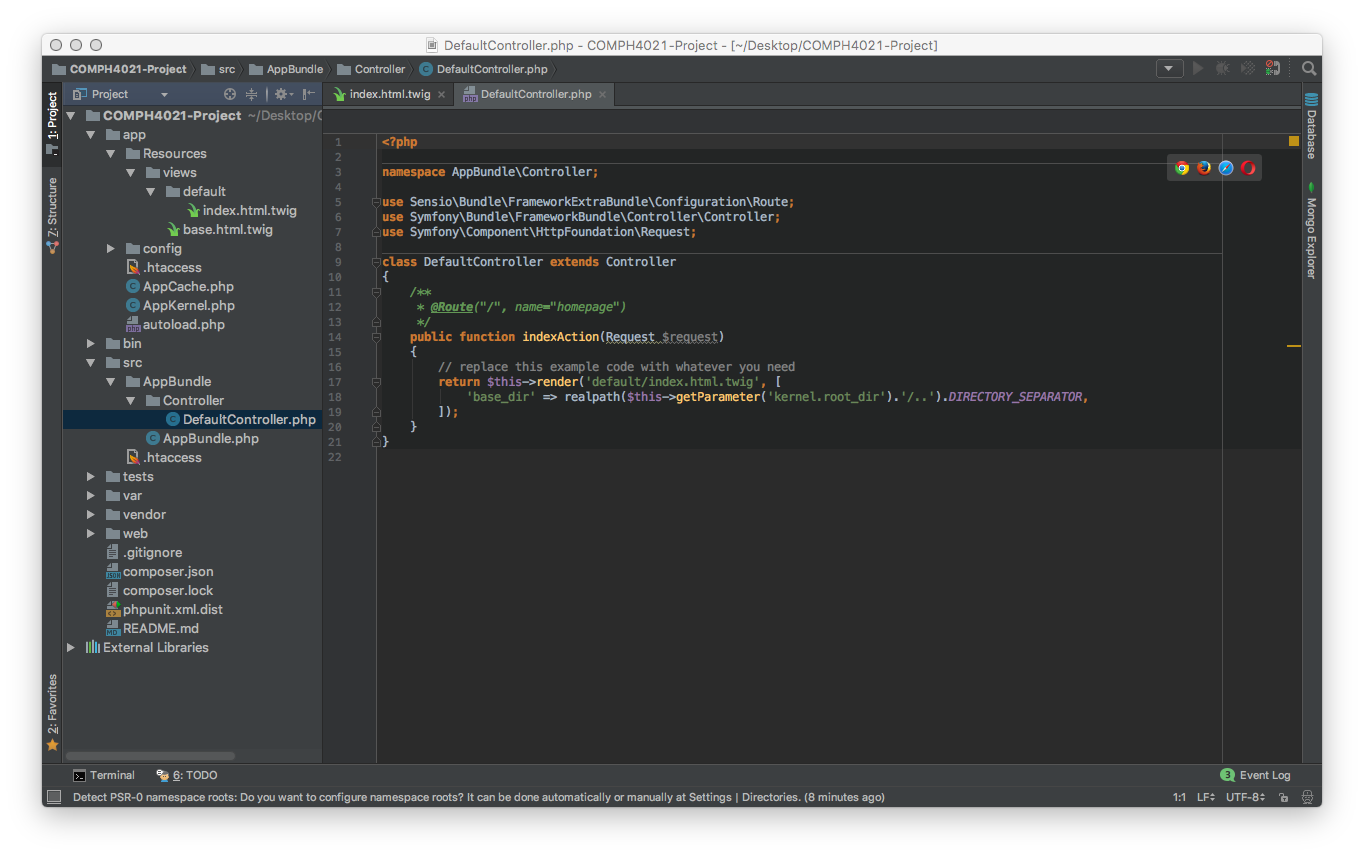
\includegraphics[width=400pt]{figures/default_controller.png} % requires the graphicx package
   \caption{Default Controller}
   \label{fig:Default Controller}
\end{figure}

Most of the files live in src/AppBundle. Looking at the controller called Default Controller in the below figure \ref{fig:Default Controller}. This controller class defines what is seen in figure \ref{fig:Symfony Browser}. It renders the Symfony Welcome Page. Take note of the @Route("/", name="homepage") annotation on line 12. It matches the route in figure \ref{fig:Web Debug Toolbar and Profiler Extended}.














%\chapter{System Design - "The How"}


\section{Introduction}

Introduce the chapter and discuss the implemention of diagrams to initiate the design

\subsection{UML Diagrams}
Design of UML diagrams
\subsection{Goals of UML}
What was achieved with using UML
\subsection{Object Oriented Approach}
fdsdfsdfds


\section{Appearance}

\subsection{Subsection header 1}
fdsdfsdfds
\subsection{Subsection header 2}
fdsdfsdfds
\subsection{Subsection header 3}
fdsdfsdfds

\section{Content}

\subsection{Subsection header 1}
fdsdfsdfds
\subsection{Subsection header 2}
fdsdfsdfds
\subsection{Subsection header 3}
fdsdfsdfds

\section{Design}

\subsection{Subsection header 1}
fdsdfsdfds
\subsection{Subsection header 2}
fdsdfsdfds
\subsection{Subsection header 3}
fdsdfsdfds

\chapter{Implementation of the System}


\section{Implementation Principles}

\subsection{Object-Oriented Approach}
How OO aided the system
\subsection{Design Patterns}
MVC withing the Netbeans IDE
\subsection{Choice of Language}
Java over PHP


\section{Stages of Admin Implementation}

\subsection{Login}
Discuss the login procedure
\subsection{Administration}
Discuss the Administation side
\subsection{Subsection header 3}
fdsdfsdfds

\section{Stages of User Implementation}

\subsection{Subsection header 1}
fdsdfsdfds
\subsection{Subsection header 2}
fdsdfsdfds
\subsection{Subsection header 3}
fdsdfsdfds

\section{Design}

\subsection{Subsection header 1}
fdsdfsdfds
\subsection{Subsection header 2}
fdsdfsdfds
\subsection{Subsection header 3}
fdsdfsdfds

\chapter{Testing and Evaluation}


\section{Introduction}
Introduction into the testing

\begin{comment}
\subsection{Subsection header 1}
fdsdfsdfds
\subsection{Subsection header 2}
fdsdfsdfds
\subsection{Subsection header 3}
fdsdfsdfds
\end{comment}


\section{Tests Conducted}
This will include do the tables work, checking encryption etc. Storing the data.

\begin{comment}
\subsection{Subsection header 1}
fdsdfsdfds
\subsection{Subsection header 2}
fdsdfsdfds
\subsection{Subsection header 3}
fdsdfsdfds
\end{comment}


\section{Algorithms}
Algorithms used to randomise the tables. And colony, traditional. The Fisher–Yates shuffle. The Knuth Fisher–Yates shuffle

\begin{comment}
\subsection{Subsection header 1}
fdsdfsdfds
\subsection{Subsection header 2}
fdsdfsdfds
\subsection{Subsection header 3}
fdsdfsdfds
\end{comment}

\section{Summary}
Summary of findings

\begin{comment}
\subsection{Subsection header 1}
fdsdfsdfds
\subsection{Subsection header 2}
fdsdfsdfds
\subsection{Subsection header 3}
fdsdfsdfds
\end{comment}
\chapter{Conclusion and Future work}


\section{Contributions}
Contributions of this project towards Faculty and the affect on the student

\begin{comment}
\subsection{Subsection header 1}
fdsdfsdfds
\subsection{Subsection header 2}
fdsdfsdfds
\subsection{Subsection header 3}
fdsdfsdfds
\end{comment}

\section{Limitations}
Limitations of project

\begin{comment}
\subsection{Subsection header 1}
fdsdfsdfds
\subsection{Subsection header 2}
fdsdfsdfds
\subsection{Subsection header 3}
fdsdfsdfds
\end{comment}


\section{Future Work}
Integrate into an undertaking currently being deployed at DCU called GURU

\begin{comment}
\subsection{Subsection header 1}
fdsdfsdfds
\subsection{Subsection header 2}
fdsdfsdfds
\subsection{Subsection header 3}
fdsdfsdfds
\end{comment}


\section{Data Collection}
Data analysis performed and exploration. As to who has submitted their examination papers

\begin{comment}
\subsection{Subsection header 1}
fdsdfsdfds
\subsection{Subsection header 2}
fdsdfsdfds
\subsection{Subsection header 3}
fdsdfsdfds
\end{comment}







\setlinespacing{1.0}
\bibliographystyle{plainnat}
\bibliography{bibliography}

\appendix
%\chapter*{Appendices}
   \nonumchapter{Appendices}

\newpage

\section{Web Application Login Screen}
\begin{comment}
\label{app:structure} \textbf{Introduction}

Dublin Bus uses electronic fareboxes
\end{comment}

\begin{figure}[htbp]
\center 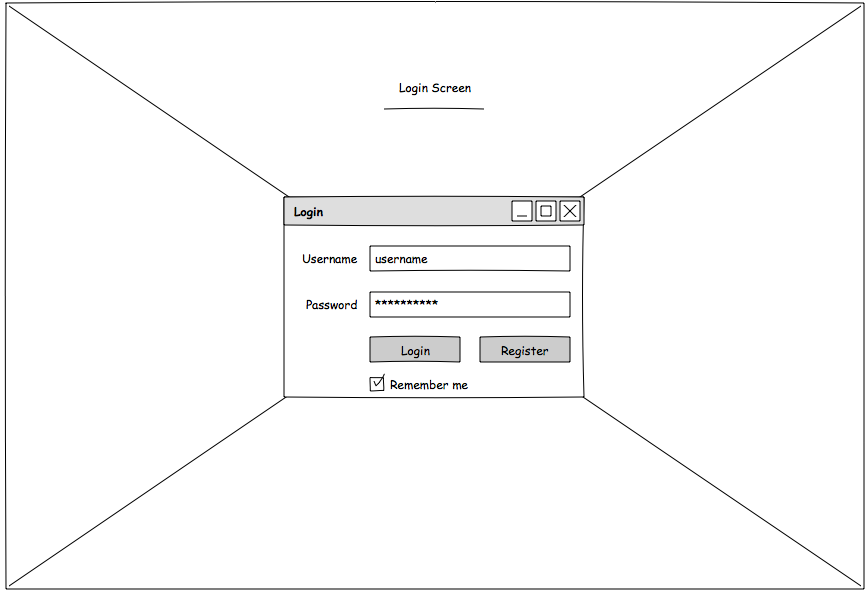
\includegraphics[width=400pt]{Figures/Login_Screen}\\
\caption{Graphical illustration of the Login Screen} \label{Figure: Graphical illustration of the Login Screen}
\end{figure}

\newpage

\section{Web Application Question Entry}
\label{Appendix: Coarse Zone Description}


\begin{comment}
\begin{longtable}
{cl} \hline
\endhead
\hline
\endfoot
\textbf{{Coarse Zone}}&
\textbf{{Coarse Zone Description}} \\
\hline \hline\textbf{{1}}&
{City Centre (within Canal Ring)} \\
\hline \textbf{{2}}&
{Dublin Port Area} \\
\hline \textbf{{3}}&
{North East City (Clontarf, Raheny, Ayrfield)} \\
\hline \textbf{{4}}&
{North West City (Cabra, Finglas, Ballymun)} \\
\hline \textbf{{5}}&
{South East City (Rathmines)} \\
\hline \textbf{{6}}&
{South West City (Kilmainham, Walkingstown, Kimmage)} \\
\hline \textbf{{7}}&
{Fingal West (Blanchardstown / Castleknock)} \\
\hline \textbf{{8}}&
{Fingal East (Portmarnock, Malahide, Donabate, Swords, Airport)} \\
\hline \textbf{{9}}&
{Fingal North West (Naul, Ballyboghill, Oldtown)} \\
\hline \textbf{{10}}&
{Fingal North East (Rush, Lusk, Skerries, Balbriggan)} \\
\hline \textbf{{11}}&
{South Dublin - Lucan, Clondalkin} \\
\hline \textbf{{12}}&
{South Dublin - Tallaght} \\
\hline \textbf{{13}}&
{South Dublin - Saggart, Rathcoole, Bohernabrena} \\
\hline \textbf{{14}}&
{Dun Laogharie / Rathdown - North} \\
\hline \textbf{{15}}&
{Dun Laoghaire / Rathdown - South} \\
\hline \textbf{{16}}&
{Meath} \\
\hline \textbf{{17}}&
{Kildare} \\
\hline \textbf{{18}}&
{West Wicklow} \\
\hline \textbf{{19}}&
{East Wicklow} \\
\hline \textbf{{20}}&
{Louth} \\
\hline \textbf{{21}}& {Externals} \label{tab1}
\end{longtable}
\end{comment}

\begin{figure}[htbp]
\center 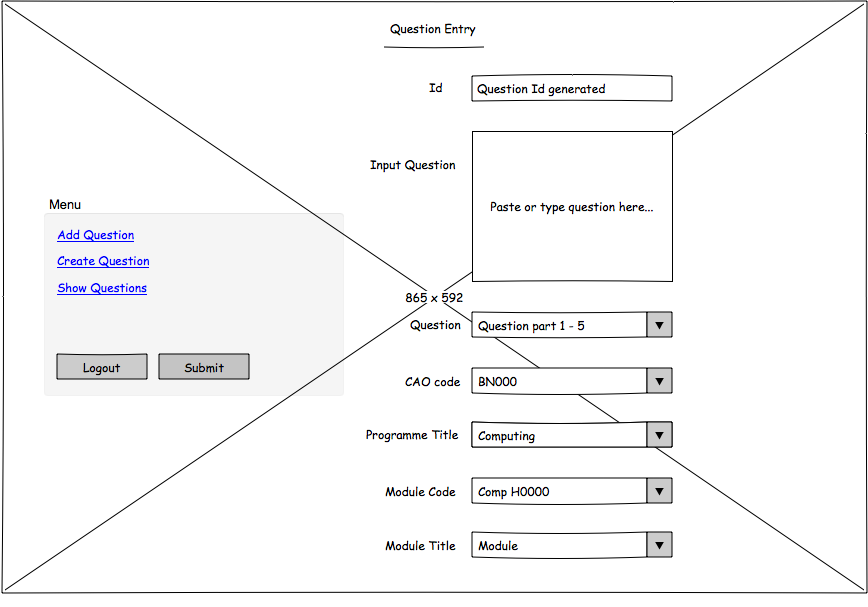
\includegraphics[width=400pt]{Figures/Question_Entry}\\
\caption{Graphical illustration of the Question Entry} \label{Figure: Graphical illustration of the Question Entry}
\end{figure}

\newpage

\section{Generate a Question}
\label{Appendix:Coarse Zone Map}

\begin{comment}
\begin{figure}[hbtp]
\center
  % Requires \usepackage{graphicx}
  \includegraphics[width=327pt]{dtomap}\\
\end{figure}
\end{comment}

\begin{figure}[htbp]
\center 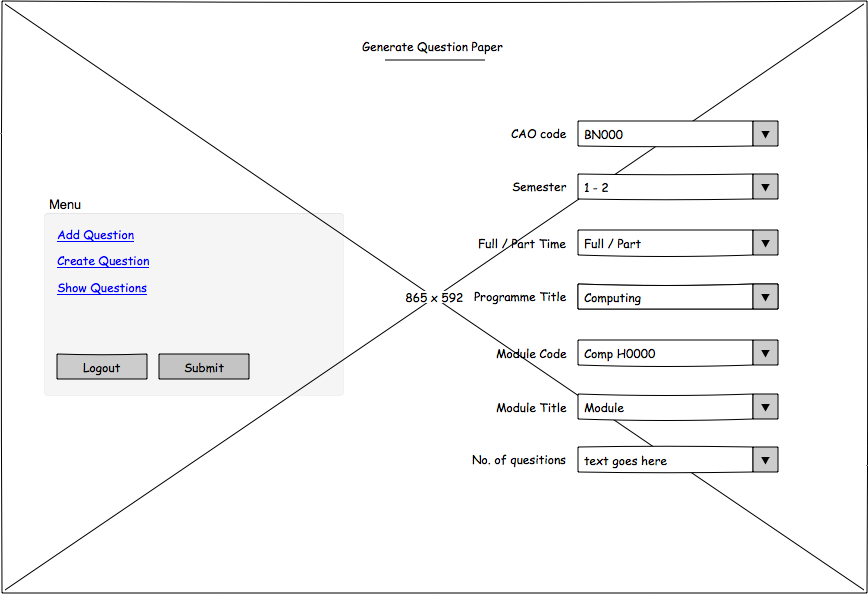
\includegraphics[width=400pt]{Figures/Generate_Question_Paper}\\
\caption{Graphical illustration of the Generate a Question Paper} \label{Figure: Graphical illustration of the Generate a Question Paper}
\end{figure}

\newpage

\section{Show questions}
\label{app:tickettypes}
\begin{comment}
\footnotesize{} \setlinespacing{1.0}
\begin{longtable}[htbp]
{cc} \hline \textbf{Ticket Type ID} & \textbf{Description} \\\hline \hline \hline
\endhead

 300&
Feeder Ticket - Child \\
\hline 301&
Feeder Ticket - Adult \\
\hline 310&
10-Journey Feeder - Adult \\
\hline 317&
Airlink Adult Airport-Busarus \\
\hline 318&
Airlink Child Airport-Busarus \\
\hline 319&
Airlink Child Airport-Heuston \\
\hline 320&
Airlink Adult Airport-Heuston \\
\hline 333&
Adult Single Feeder \\
\hline 365&
Child Bus/Rail Short Hop - Day \\
\hline 366&
Adult Bus/Rail Short Hop - Day \\
\hline 367&
Family Bus/Rail Short Hop - Day \\
\hline 369&
4 Day Explorer \\
\hline 410&
Weekly Adult Short Hop Bus/Rail \\
\hline 430&
Weekly Adult Medium Hop Bus/Rail \\
\hline 431&
Weekly Adult Long Hop Bus/Rail \\
\hline 432&
Weekly Adult Giant Hop Bus/Rail \\
\hline 433&
Monthly Adult Short Hop Bus/Rail \\
\hline 455&
Monthly Adult Long Hop Bus/Rail \\
\hline 456&
Monthly Adult Giant Hop Bus/Rail \\
\hline 457&
Monthly Student Short Hop Bus/Rail \\
\hline 458&
Annual Bus/Rail \\
\hline 478&
Annual All CIE Services \\
\hline 479&
Annual CIE Pensioner Bus/Rail \\
\hline 480&
Monthly CIE Pensioner Bus/Rail \\
\hline 493&
Foreign Student - 1 Week \\
\hline 494&
Foreign Student - 2 Week \\
\hline 495&
Foreign Student - 3 Week \\
\hline 496&
Foreign Student - 4 Week \\
\hline 497&
CYC Group \\
\hline 600&
Adult Cash Fare \\
\hline 608&
Nitelink (Maynouth/Celbridge) \\
\hline 609&
Nitelink (Maynouth/Celbridge) \\
\hline 610&
Child Cash Fare \\
\hline 620&
Schoolchild Cash Fare \\
\hline 625&
Adult (formerly Shopper) \\
\hline 630&
Adult 10-Journey (3 Stages) \\
\hline 631&
Adult 10-Journey (7 Stages) \\
\hline 632&
Adult 10-Journey (12 Stages) \\
\hline 633&
Adult 10-Journey (23 Stages) \\
\hline 634&
Adult 10-Journey (23+ Stages) \\
\hline 640&
Adult 2-Journey (3 Stages) \\
\hline 641&
Adult 2-Journey (7 Stages) \\
\hline 642&
Adult 2-Journey (12 Stages) \\
\hline 643&
Adult 2-Journey (23 Stages) \\
\hline 644&
Adult 2-Journey (23+ Stages) \\
\hline 650&
Schoolchild 10-Journey \\
\hline 651&
Scholar 10-Journey \\
\hline 652&
Schoolchild 2-Journey \\
\hline 653&
Scholar 2-Journey \\
\hline 657&
Transfer 90 (or Passenger Change) \\
\hline 658&
Adult Single Heuston-CC \\
\hline 660&
Adult One Day Travelwide \\
\hline 661&
Child One Day Travelwide \\
\hline 662&
Family One Day Travelwide \\
\hline 665&
Rambler (3 Day Bus only) \\
\hline 670&
Weekly Adult Bus \\
\hline 671&
Weekly Adult Cityzone \\
\hline 690&
Weekly Student Travelwide \\
\hline 691&
Weekly Student Cityzone \\
\hline 705&
Monthly Adult Citizone (AerLingus.) \\
\hline 710&
Monthly Adult Travelwide \\
\hline 730&
Annual Adult Travelwide \\
\hline 760&
Annual Staff Bus \\
\hline 790&
School Pass \\
\hline 791&
OAP Pass \\
\hline 800&
City Tour - Adult \\
\hline 801&
City Tour - Family \\
\hline 802&
City Tour - Child \\
\hline 898& 10 - Journey Test Ticket \\\hline \label{tab1}
\end{longtable}
 \normalsize{} \setlinespacing{1.1}
\end{comment}

\begin{figure}[htbp]
\center 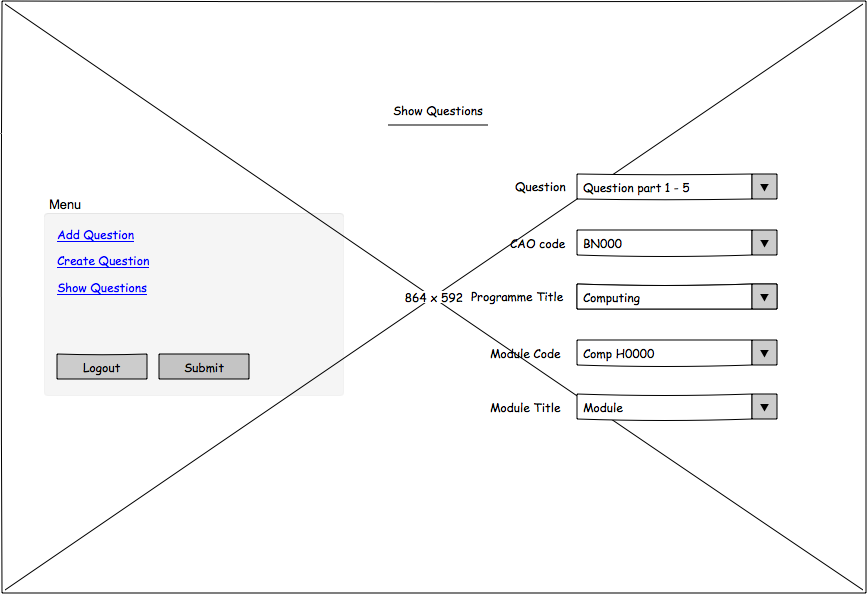
\includegraphics[width=400pt]{Figures/Show_Questions}\\
\caption{Graphical illustration of the Menu List to view the Questions} \label{Figure: Graphical illustration of the Menu List to view the Questions}
\end{figure}

\newpage

\section{Show}
\label{Appendix: Ticket 1 -- 730-243}

\begin{comment}
\footnotesize{} \setlinespacing{1.0} \vspace{10pt}

\begin{longtable}[htbp] {ccccccc} \hline
\textbf{Date}& \textbf{Stage}& \textbf{Boarding Time}&

\textbf{Route}   & \textbf{Direction}& \textbf{Zone}&
\textbf{Area} \\
\hline \hline 01/10/1999& 62& 08:03&

150   & 1& 12&
Templeogue \\
\hline 01/10/1999& 25& 18:26&

150   & 0& 1&
City Centre South \\
\hline 02/10/1999& 70& 10:03&

16   & 1& 6&
Harolds Cross \\
\hline 02/10/1999& 25& 14:38&

16   & 0& 1&
City Centre North \\
\hline 04/10/1999& 62& 08:29&

150   & 1& 12&
Templeogue \\
\hline 04/10/1999& 25& 18:37&

150   & 0& 1&
City Centre South \\
\hline 05/10/1999& 62& 08:07&

150   & 1& 12&
Templeogue \\
\hline 05/10/1999& 25& 17:21&

150   & 0& 1&
City Centre South \\
\hline 06/10/1999& 62& 07:49&

150   & 1& 12&
Templeogue \\
\hline 06/10/1999& 25& 17:25&

150   & 0& 1&
City Centre South \\
\hline 08/10/1999& 62& 08:12&

150   & 1& 12&
Templeogue \\
\hline 08/10/1999& 25& 18:13&

150   & 0& 1&
City Centre South \\
\hline 11/10/1999& 62& 08:37&

150   & 1& 12&
Templeogue \\
\hline 11/10/1999& 25& 18:12&

150   & 0& 1&
City Centre South \\
\hline 12/10/1999& 62& 07:27&

150   & 1& 12&
Templeogue \\
\hline 12/10/1999& 25& 14:47&

150   & 0& 1&
City Centre South \\
\hline 13/10/1999& 62& 08:17&

150   & 1& 12&
Templeogue \\
\hline 13/10/1999& 25& 13:34&

150   & 0& 1&
City Centre South \\
\hline 16/10/1999& 70& 08:07&

65B   & 1& 5&
Rathmines \\
\hline 16/10/1999& 25& 12:47&

16   & 0& 1&
City Centre North \\
\hline 19/10/1999& 62& 08:10&

150   & 1& 12&
Templeogue \\
\hline 19/10/1999& 25& 16:28&

150   & 0& 1&
City Centre South \\
\hline 20/10/1999& 62& 08:13&

150   & 1& 12&
Templeogue \\
\hline 20/10/1999& 25& 18:22&

150   & 0& 1&
City Centre South \\
\hline 21/10/1999& 62& 08:09&

150   & 1& 12&
Templeogue \\
\hline 21/10/1999& 25& 16:17&

150   & 0& 1&
City Centre South \\
\hline 22/10/1999& 62& 08:14&

150   & 1& 12&
Templeogue \\
\hline 22/10/1999& 25& 17:45&

150   & 0& 1&
City Centre South \\
\hline 27/10/1999& 62& 08:11&

150   & 1& 12&
Templeogue \\
\hline 27/10/1999& 25& 17:36&

150   & 0& 1&
City Centre South \\
\hline 28/10/1999& 62& 08:18&

150   & 1& 12&
Templeogue \\
\hline 28/10/1999& 25& 17:47&

150   & 0& 1&
City Centre South \\
\hline 29/10/1999& 62& 08:00&

150   & 1& 12&
Templeogue \\
\hline 29/10/1999& 25& 18:07&

150   & 0& 1&
City Centre South \\
\hline 30/10/1999& 70& 09:15&

16A   & 1& 6&
Harolds Cross \\
\hline 30/10/1999& 25& 14:53&

155   & 0& 0& City Centre South \\ \hline \label{tab14}
\end{longtable}
 \normalsize{} \setlinespacing{1.1}
\end{comment}

\begin{figure}[htbp]
\center 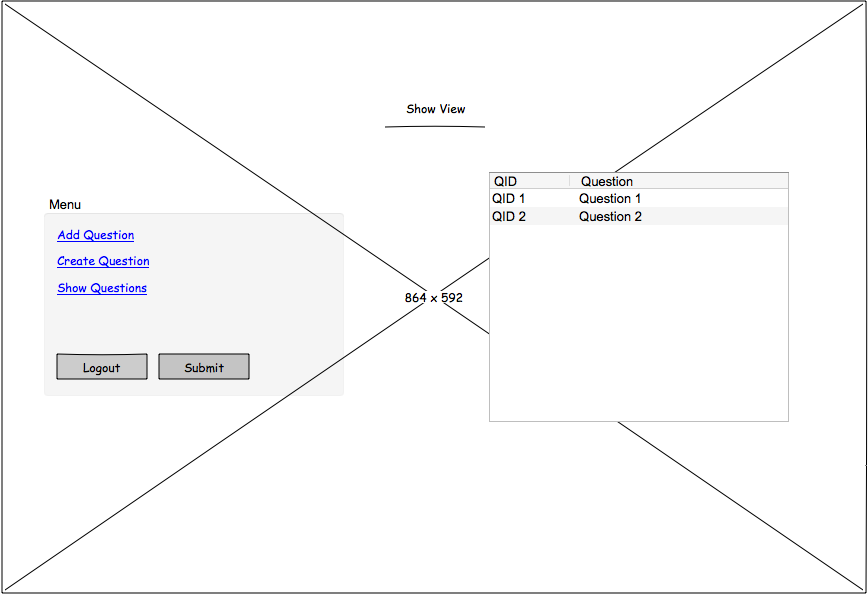
\includegraphics[width=400pt]{Figures/Shows}\\
\caption{Graphical illustration of the Show list} \label{Figure: Graphical illustration of the Show list}
\end{figure}

\begin{comment}
\newpage

\section{Ticket 3 -- 730-73}
\label{Appendix: Ticket 3 -- 730-73}

\footnotesize{} \setlinespacing{1.0} \vspace{10pt}  \begin{longtable}[htbp] {ccccccc} \hline
\textbf{Date}& \textbf{Stage}& \textbf{Boarding Time}& \textbf{Route}& \textbf{Direction}&
\textbf{Zone}&
\textbf{Area} \\
\hline \hline 01/10/1999& 15& 07:45& 130& 1& 3&
Clontarf \\
\hline 01/10/1999& 75& 17:17& 130& 0& 1&
City Centre North \\
\hline 04/10/1999& 14& 07:49& 130& 1& 3&
Clontarf \\
\hline 04/10/1999& 75& 17:36& 130& 0& 1&
City Centre North \\
\hline 05/10/1999& 14& 07:55& 130& 1& 3&
Clontarf \\
\hline 05/10/1999& 75& 17:22& 130& 0& 1&
City Centre North \\
\hline 06/10/1999& 13& 07:42& 130& 1& 3&
Clontarf \\
\hline 06/10/1999& 75& 17:28& 130& 0& 1&
City Centre North \\
\hline 08/10/1999& 14& 07:56& 130& 1& 3&
Clontarf \\
\hline 08/10/1999& 75& 17:32& 130& 0& 1&
City Centre North \\
\hline 11/10/1999& 15& 07:43& 130& 1& 3&
Clontarf \\
\hline 11/10/1999& 75& 17:24& 130& 0& 1&
City Centre North \\
\hline 12/10/1999& 15& 07:53& 130& 1& 3&
Clontarf \\
\hline 12/10/1999& 75& 17:26& 130& 0& 1&
City Centre North \\
\hline 13/10/1999& 15& 07:53& 130& 1& 3&
Clontarf \\
\hline 13/10/1999& 75& 17:28& 130& 0& 1&
City Centre North \\
\hline 14/10/1999& 15& 07:58& 130& 1& 3&
Clontarf \\
\hline 14/10/1999& 75& 18:51& 130& 0& 1&
City Centre North \\
\hline 15/10/1999& 15& 07:53& 130& 1& 3&
Clontarf \\
\hline 15/10/1999& 75& 17:10& 130& 0& 1&
City Centre North \\
\hline 20/10/1999& 14& 07:46& 130& 1& 3&
Clontarf \\
\hline 20/10/1999& 75& 17:29& 130& 0& 1&
City Centre North \\
\hline 21/10/1999& 15& 08:07& 130& 1& 3&
Clontarf \\
\hline 21/10/1999& 75& 18:39& 130& 0& 1&
City Centre North \\
\hline 22/10/1999& 16& 08:07& 130& 1& 3&
Clontarf \\
\hline 22/10/1999& 75& 17:01& 130& 0& 1&
City Centre North \\
\hline 26/10/1999& 15& 07:51& 130& 1& 3&
Clontarf \\
\hline 26/10/1999& 75& 17:36& 130& 0& 1&
City Centre North \\
\hline 27/10/1999& 15& 07:52& 130& 1& 3&
Clontarf \\
\hline 27/10/1999& 75& 17:34& 130& 0& 1&
City Centre North \\
\hline 28/10/1999& 15& 08:09& 130& 1& 3&
Clontarf \\
\hline 28/10/1999& 75& 18:34& 130& 0& 1&
City Centre North \\
\hline 29/10/1999& 14& 07:59& 130& 1& 3&
Clontarf \\
\hline 29/10/1999& 75& 17:21& 130& 0& 1& City Centre North \\ \hline \label{tab16}
\end{longtable}
 \normalsize{} \setlinespacing{1.1}
\end{comment}

\newpage




\end{document}
% ------------------------------------------------------------------------
%%%      \setlength\LTleft{1pt}
